\documentclass[10pt,journal,letterpaper]{IEEEtran}
\usepackage[T1]{fontenc}
\usepackage[utf8]{inputenc}
\usepackage{amsmath,amssymb,booktabs,graphicx,tabularx,microtype}
\usepackage{cite}
\usepackage[hidelinks]{hyperref}
\usepackage{placeins}
\interdisplaylinepenalty=2500
\emergencystretch=1.5em

% Retain natural table text size and shrink only when necessary.
\newsavebox{\ArticleTableBox}
\newcommand{\FitTable}[1]{%
  \sbox{\ArticleTableBox}{#1}%
  \ifdim\wd\ArticleTableBox>\linewidth
    \resizebox{\linewidth}{!}{\usebox{\ArticleTableBox}}%
  \else
    \usebox{\ArticleTableBox}%
  \fi
}

\hypersetup{pdftitle={Microservice Resource Forecasting under Incomplete Telemetry: Decomposition, Compact Models and Calibrated Transfer},pdfauthor={Carlos Augusto Mullisaca Condori; Jhon Alex Gutiérrez Morales}}
\title{Microservice Resource Forecasting under Incomplete Telemetry: Decomposition, Compact Models and Calibrated Transfer}
\author{Carlos~Augusto~Mullisaca~Condori and Jhon~Alex~Gutiérrez~Morales%
  \thanks{School of Systems Engineering, Faculty of Engineering and Architecture, Universidad Peruana Unión, Juliaca, Peru. Email: \mbox{\nolinkurl{carlos.mullisaca@upeu.edu.pe}} and \mbox{\nolinkurl{alex.gutierrez@upeu.edu.pe}}. Corresponding author pending designation.}}

\begin{document}
\maketitle
\begin{abstract}
Incomplete telemetry complicates microservice resource forecasting and can change the accuracy gained from more complex models. We examine how temporal decomposition, availability descriptors and model size affect CPU and memory forecasts across five experimental phases. The historical ChronoGraph experiment uses 28 services, 8005 timestamps, a chronological 70/10/20 split, twelve-step histories, three training seeds and twenty paired masks. Experiments with E0--E5 and compact C0--C3/V2 motivate calibrated transfer to 32 additional services. The expanded comparison evaluates fifteen families with ten primary neural seeds and twenty masks. Secondary experiments vary missingness, direct horizons and history lengths. Frozen models also transfer to one day of Alibaba 2022 after six hours of calibration. Historically, E5 reduces paired memory MASE by 1.280\% relative to DLinear and increases CPU MASE by 0.984\%. V2 does not retain the full memory gain. On the additional services, A3 uses 15 parameters and improves memory MASE by 0.02523 relative to E5's 74-parameter configuration. All ten seed means favor A3 (Holm-adjusted exact sign-test $p=0.0078125$), with improvement in only 10 of 32 services. A3 does not generally improve on DLinear. Small PatchTST and NLinear have the lowest observed primary MASE means, while persistence ranks first externally. A3 achieves CPU/CUDA median forward times of 0.050/0.141 ms with resident inputs for one origin and 32 services. The results establish context-specific tradeoffs under synthetic loss, shared ChronoGraph periods and short external coverage.

\end{abstract}
\begin{IEEEkeywords}
Microservices, forecasting, incomplete telemetry, DLinear, calibrated transfer, reproducibility.
\end{IEEEkeywords}

\section{Introduction}
Microservice resource forecasts can provide inputs to capacity planning and autoscaling, but a forecast of recorded CPU or memory usage does not directly estimate unconstrained demand or demonstrate a better controller. Telemetry can be unavailable when collectors, transport or services fail. A forecaster must then separate the last observed value from the availability of that value, and its computational cost must remain appropriate for the monitoring setting. Work on workload learning, decomposition-based autoscaling and resource forecasting provides the application context \cite{powerprediction,autoscaling2025,temposcale,aero}. The present study evaluates point forecasts; it does not implement a controller or measure energy, service-level violations or cloud bills.

A second motivation concerns the interpretation of temporal decomposition. DLinear combines affine predictions from a fixed moving-average trend and its residual \cite{dlinear}. With a fixed linear smoothing operator, their sum is an affine function of the input window. Reducing the parameterization therefore need not introduce a new function class. Availability-dependent smoothing and explicit missingness descriptors are different interventions, and empirical gains cannot be inferred from either algebraic equivalence or a smaller parameter count. This distinction is particularly relevant when a small model is presented as an architectural improvement.

This work extends an existing, already inspected experiment on 28 ChronoGraph services. All historical artifacts remain separate from new evidence. We evaluate source-trained models on 32 additional services, with prefix-only destination calibration, and on a short external Alibaba 2022 case. The source and additional services share an infrastructure and observation period. Consequently, the primary evaluation is a predeclared spatial-transfer experiment, not an independently blinded temporal replication. An immutable local protocol and checkpoint freezes precede the corresponding target evaluations; they are not a public preregistration.

The contribution is an auditable empirical study rather than a claim of a universally superior architecture. It comprises (i) a compact affine parameterization with two separately ablated availability descriptors; (ii) paired evaluation of 15 families under ten missingness conditions, with ten seeded neural fits in the primary setting; (iii) direct-horizon and history-length extensions, plus calibrated external transfer; and (iv) independently reconstructed saved-prediction metrics and measured CPU/CUDA inference costs. Negative outcomes and limitations are retained.

\subsection{Research questions and evidence boundaries}
The research questions are: RQ1, how do error levels change with incomplete telemetry? RQ2, how do fixed decomposition, availability-dependent smoothing and compact parameterizations trade accuracy against cost? RQ3, when are missing-fraction and age descriptors useful? RQ4, does a compact affine model retain accuracy with fewer parameters? RQ5, how do conclusions change across services, direct horizons and datasets? RQ6, how much variation occurs across seeded fits, masks and time periods?

The operational primary hypothesis compares A3 with DLinear and E5 separately for CPU and memory. Four two-sided contrasts were specified; no improvement is required for completion. Missingness monotonicity, descriptor ablations, added stress mechanisms, horizon/history effects and external transfer are descriptive secondary analyses. The historical experiment motivated these hypotheses and remains exploratory. Fig.~\ref{fig:flow} summarizes the separation of evidence.
\begin{figure*}[!t]\centering
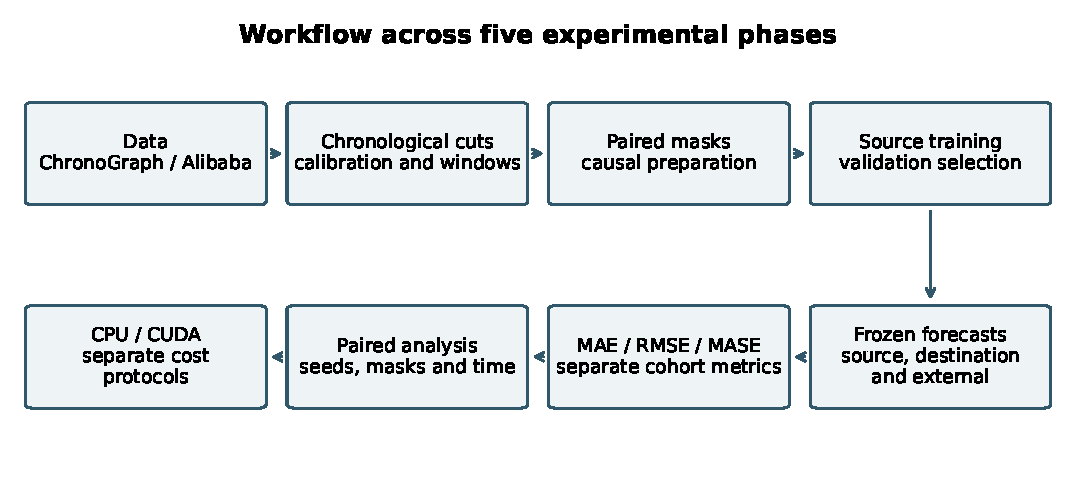
\includegraphics[width=0.93\textwidth]{figuras/01_methodology.pdf}
\caption{Study flow. Model selection and weights use only the 28-service source training/validation periods. The 32 destination services supply their training-prefix calibration statistics, not destination fitting or hyperparameter selection. Alibaba uses a separate six-hour calibration prefix.}\label{fig:flow}
\end{figure*}

\subsection{An integrated sequence of five experimental phases}
The study began with a specific intervention in a lightweight forecasting model: changing its decomposition and distinguishing an observed measurement from a carried or fallback value. This starting point is useful because an imputed scalar alone does not identify the measurement process that generated it. Nevertheless, representing that process increases capacity and can encourage a model to fit the synthetic generator. A successful missingness descriptor must therefore justify itself through both held-out error and computational measurements. The historical E0--E5 experiments established the initial empirical question; compact variants tested whether a smaller summary could preserve the apparent benefit; additional comparators and service cohorts subsequently tested its portability.

The five phases are complementary rather than independent replications. Phase I examines temporal decomposition and missingness heads on the fixed 28-service source cohort. Phase II evaluates C0--C3 and the validation-selected alias V2 on that same known test. Phase III refits source models under the expanded protocol and transfers them to 32 additional services. Phase IV stresses these models with additional mechanisms, direct horizons, longer histories and a separate short Alibaba case. Phase V measures computation in the actual implementations. The narrative follows the progression of the scientific question, while the chronology of test exposure remains part of the validity analysis.

In particular, the source-test observation that E5 helped memory motivated subsequent model development. The new-service protocol froze four primary contrasts before evaluating those destination outcomes, but the source period was already familiar. Consequently, the locally frozen contrasts improve procedural transparency without making the entire project prospectively blinded. An effect can be consistent across initializations of a fixed model and still fail to extend across services or datasets. Maintaining these distinctions is necessary to explain why compactness, seed consistency and transfer accuracy need not agree.

The research gap addressed here is a joint empirical accounting of decomposition, measurement provenance, capacity and transfer under one recorded pipeline. It is narrower than proposing a general solution to cloud resource management. Forecasting measured usage supplies one input to a future management decision, whereas a controller also requires a policy, capacity constraints and an action-dependent system response. The implemented experiments assess point error and execution cost. They cannot identify how unobserved demand would respond to allocating more resources, and they do not estimate the monetary value of a small MASE change.

\section{Related work and theoretical foundations}
Linear forecasting remains a necessary reference in comparisons with deep temporal models. DLinear and NLinear question whether architectural complexity alone explains forecasting accuracy \cite{dlinear}. PatchTST uses channel-independent patches for Transformer forecasting \cite{patchtst}; TimesNet represents temporal variation in two dimensions \cite{timesnet}; iTransformer places variates in the token dimension \cite{itransformer}; TiDE uses dense temporal encoding \cite{tide}; and TimeMixer combines information across temporal scales \cite{timemixer}. These methods have different benchmark recipes and budgets. We execute a small official-code PatchTST configuration as a feasible modern comparator, without transferring published accuracy claims to our protocol. The other architectures are reviewed rather than reported as executed experiments.

Rubin distinguishes missingness mechanisms by the information on which availability depends \cite{rubinmissing}. The lag-based mask here is a specified simulation based on past observations. Missingness-aware recurrent models use both observations and the measurement process. GRU-D introduces input and hidden-state decay \cite{grud}; our shared-service adaptation is not a reproduction of its clinical multivariate setting. Graph-based forecasting with missing values is addressed by BiTGraph \cite{bitgraph} and GinAR \cite{ginar}. Their historical implementations and results are preserved, including very large errors, but are not newly fitted in every transfer scenario. The two GRU comparators in the new experiment test local information and static neighborhood aggregation, using the recurrent cell of \cite{gru}. The ChronoGraph project combines microservice temporal data and call relationships \cite{chronograph}; a known static graph is treated as an input assumption, not as proof that every edge was available at every historical forecast origin.

Cloud-specific studies distinguish the prediction target and the action taken from it. TempoScale concerns microservice autoscaling \cite{temposcale}, AERO includes adaptive period detection in resource prediction \cite{aero}, and STAMP integrates system state and spatiotemporal dependencies for microservice workload prediction \cite{stamp}. Broader reviews discuss AI applications to microservices and autoscaling methods \cite{aimapping,autoscaling2025}. Our authors' recent systematic review provided candidate references; the primary publications were checked separately before inclusion. Its counts of papers are not counts of experiments in this study. Further work on missing-variable forecasting, dynamic telemetry sampling, adaptive microservice management and cloud anomaly detection provides adjacent context, with preprint or under-review status recorded where applicable \cite{ibn,radar2026,taxonomy2026,ibm2026}. Anomaly-detection scores are not directly comparable with forecasting MASE.

STEAM builds a graph from workload similarity and uses system-state information to create alternative graph views \cite{steamgraph}. This provides a point of comparison for the static call adjacency used here. DeepScaling evaluates a scaling policy that targets stable CPU utilization \cite{deepscaling}. Its unit of evaluation includes control decisions, whereas this study measures forecast error on recorded usage.

Finally, uncertainty about a measured mean difference is distinct from uncertainty about an individual future observation. We report conditional resampling intervals for algorithm comparisons using temporal blocks \cite{blockbootstrap}. We do not construct prediction intervals or claim coverage; conformal prediction introduces additional assumptions and calibration decisions beyond these experiments \cite{conformal}. MASE is used as a scale-normalized error with a training-prefix denominator \cite{mase}; it does not remove differences in target semantics between the two data sources.


\subsection{Forecasting targets, decomposition and incomplete histories}
A multivariate infrastructure dataset does not require every predictor to use all its variables jointly. Here CPU and memory are separate supervised targets, and most linear predictors share coefficients across services while consuming one service's resource history. The graph recurrent comparator introduces neighboring services through fixed incoming and outgoing aggregates. Thus the source data are multivariate, but an individual linear forecast is a shared univariate mapping after service-specific calibration. This distinction prevents a low-cost per-service head from being described as a learned joint model of the complete infrastructure.

A temporal decomposition separates a smoothed level from a residual \cite{hyndmanfpp3}. Neither the residual nor a high autocorrelation at a daily lag establishes seasonality. The MA25 reference uses repeated endpoints on a twelve-step history, which makes padding an important part of its implemented transformation. Exponential smoothing instead updates a state with geometrically declining influence, and the availability-aware version skips measurement updates when the input is imputed. Persistence, moving average and observation-updated exponential smoothing are also evaluated as direct statistical predictors. A decomposition inside a trained head and an exponential-smoothing predictor are different models even when they use similar recurrences.

NLinear subtracts the last prepared input value before an affine projection and adds that value back to the output. This normalization makes a recent level explicit, but the recent value may itself be carried forward under missingness. Its competitiveness therefore does not demonstrate recovery of hidden measurements. Ridge provides a regularized affine reference fitted analytically \cite{hoerlkennard}. The single-head A0 provides a gradient-trained affine reference initialized from the two DLinear heads. Differences among their predictions may reflect initialization, loss, regularization and selection rather than different expressive power on complete filled histories.

Missing-data treatment has two roles. Causal filling supplies a numerical input; provenance channels tell the predictor whether it is measured or substituted. Age summarizes the length of a missing run and can become large even with a short explicit input window. The synthetic lag-MAR mechanism additionally links observation probability to a previously available CPU state. This creates an implemented observation process whose rate differs from its nominal label. It does not establish that real collector failures are missing at random, nor does it justify conditioning a generator on hidden contemporaneous CPU.

GRU cells encode a sequence through gated state updates \cite{gru}. GRU-D extends recurrent modeling with measurement indicators and decay \cite{grud}; its shared-service adaptation here is intentionally identified as an adaptation. Graph methods can exploit service relationships, but adjacency is not synonymous with a known causal influence. BiTGraph and GinAR are retained in historical comparisons \cite{bitgraph,ginar}. PatchTST represents input subsequences as patches and applies attention \cite{patchtst}; the small executed recipe provides a feasible comparator, not a claim to exhaust Transformer forecasting. Table~\ref{tab:related} distinguishes implemented families from bibliographic context.

\begin{table*}[!t]
\caption{State-of-the-art context and implemented scope. Published results from different tasks are not combined with the present measurements.}\label{tab:related}
\centering\footnotesize
\begin{tabularx}{\linewidth}{p{.23\linewidth}XX}
\toprule Work/family & Relevant mechanism & Execution and boundary \\\midrule
DLinear/NLinear \cite{dlinear} & Affine forecasting and explicit level handling & Executed; short histories and source-only selection \\
GRU/GRU-D \cite{gru,grud} & Gating, availability and decay & Executed adaptations; no clinical-task reproduction \\
BiTGraph/GinAR \cite{bitgraph,ginar} & Graph and incomplete-variable forecasting & Historical only; local budget and missingness task \\
PatchTST \cite{patchtst} & Channel-independent temporal patches & Small executed configuration, not published recipe \\
TimesNet, iTransformer, TiDE, TimeMixer \cite{timesnet,itransformer,tide,timemixer} & Alternative temporal representations & Reviewed only; no experimental ranking here \\
Cloud prediction \cite{powerprediction,temposcale,aero,stamp} & Prediction integrated with resource management & Context; no controller outcome measured here \\
\bottomrule
\end{tabularx}
\end{table*}

\section{Methodology}
\subsection{Historical evidence and data provenance}
Table~\ref{tab:master} summarizes the executed design. The preserved historical study contains 8005 shared time rows, CPU and memory, 28 services, a 12-step input and one-step (30-minute) forecast. It uses three training seeds, twenty mask realizations and seven conditions: complete telemetry and scattered/short-block losses at 10\%, 20\% and 40\%. Its E0--E5, C0--C3, V2 and original comparators remain available. V2 selects an already trained compact family using source validation; it is not an additional independently trained model. A historical prediction-manifest audit checks the preserved files. Their errors must not be combined with new-service errors as if the two cohorts were independent replications.

ChronoGraph provides nominally half-hour samples. The publisher describes 708 services and 1529 edges in the full graph \cite{chronograph}. The analyzed cohorts are induced subsets, with no use of all 708 services for model fitting. We retain chronological row cuts $[0,5603)$, $[5603,6404)$ and $[6404,8005)$, giving 70/10/20 proportions to rounding. These proportions refer to rows, not elapsed wall time: one 108000-second jump occurs after row 5907 in validation. Windows and MASE consecutive pairs do not cross that gap. The source cohort is unchanged. Its induced subgraph retains 28 internal edges and excludes 137 boundary edges. A separate 32-service cohort is chosen using static topology and a reproducible SHA-ranked traversal, excluding the original 28 services and four known pilot services. Selection does not use forecast errors. This connected convenience cohort is not a random sample of microservice populations.

All weights and hyperparameters use source training/validation only. For each destination service, mean, standard deviation, median and the MASE denominator use its first 5603 rows. Destination validation rows do not select models. This is \emph{calibrated spatial transfer}: it is not strict zero-shot forecasting without destination data. CPU stays on the publisher's scale; memory is in bytes. No conversion to CPU cores or percentage is assumed. The static destination graph supplies new adjacency buffers for graph models, with no new learned weights. Its edge-availability dates are not fully established.

The external case uses the first 48 official Alibaba 2022 \texttt{MSMetricsUpdate} objects, covering one day \cite{alibaba2022}. The source archive totals 17,890,753,336 bytes and 675,424,445 pod CSV rows. A bounded download queue checks the owner's Content-MD5 values and records SHA-256 values. Thirty-two service names are chosen by a SHA ranking among services covering every timestamp in the initial object; they are then placed in lexicographic order. Selection uses availability rather than forecast performance. For each timestamp, pod values with both resource fields finite are averaged by service. Those timestamp means receive equal weight in a completed half-hour bin. Bins with fewer than 30 valid minute observations are missing. Their means become available only at bin close, so no future bin values enter an input.

Alibaba's published resource values are min--max normalized utilization, not physical cores or bytes. The temporal scope of the provider's normalization is undocumented here. The processed case has 48 bins; the first 12 bins (six hours) supply calibration statistics and may appear in past input windows. The remaining 36 bins are forecast targets. Four scalar values are naturally missing in calibration only, corresponding to two service/bin pairs in both resources; no evaluation target is imputed. Frozen L12, one-step source weights are transferred without external fitting or tuning. GRU with graph is excluded because the external call graph was not acquired. This external design is deliberately distinct from the 70/10/20 source experiment and supplies only a short, exploratory cross-dataset case.

\subsection{Causal preparation and synthetic missingness}
Let $y_{t,s,r}$ be the recorded target at time $t$, service $s$ and resource $r$. Each resource is forecast separately. The input contains $L$ prepared steps ending at $t-h$, and the direct scalar output predicts $y_{t,s,r}$. Partition boundaries and temporal gaps reset the preparation. Normalization uses the corresponding training-prefix statistics; the standard deviation has a numerical floor of $10^{-8}$. Calibration statistics precede synthetic masking. The study therefore does not test learning those statistics from synthetically degraded calibration data.

At each step, an observed value is retained, a missing value uses the last available observation, and the training median is used until the first observation in the segment. Define $m$ as the observation indicator, $c$ as missing-after-an-observation and $f$ as missing-before-any-observation; $m+c+f=1$. The age $\delta$ counts missing steps since the latest available sample. Prepared channels contain the filled normalized value, $m$, $\log(1+\delta)/\log(1+L)$, $c$ and $f$. Inputs contain no target-time information. However, the propagated value and its age can summarize an observation older than the nominal $L$-step window; $L$ is not a strict upper bound on historical information.

Seven original conditions are retained. Scattered losses select an exact rounded number of unavailable entries per service/segment. Short-block losses allocate that count using candidate blocks of at most six steps. Three additional conditions use nominal 20\% loss: correlated masks shared within consecutive lexicographic groups of eight services; prolonged candidate blocks of at most 24 steps; and lag-dependent MAR. The block construction leaves separators and can truncate the final selected block to meet the exact count. These are simulated monitoring mechanisms, not recorded outages.

The lag-MAR probability at a step is
\begin{equation}
 p_t=0.2\{1+0.5\tanh(|z^{\mathrm{last,CPU}}_t|)\},
\end{equation}
where $z^{\mathrm{last,CPU}}_t$ is based on the latest \emph{previously observed} normalized CPU. Thus $0.2\leq p_t<0.3$; ``20\%'' is a nominal condition label, not its realized rate. A shared induced mask applies to both resources, intersected with their natural availability. Twenty paired mask seeds are used in the primary setting, identically across model families and training seeds. Their sequence was already used historically; new-service evaluation does not make that sequence unseen. Fig.~\ref{fig:masks} displays actual generated masks. Fig.~\ref{fig:temporal} illustrates the cut positions and forecast origin.

\begin{figure*}[t]\centering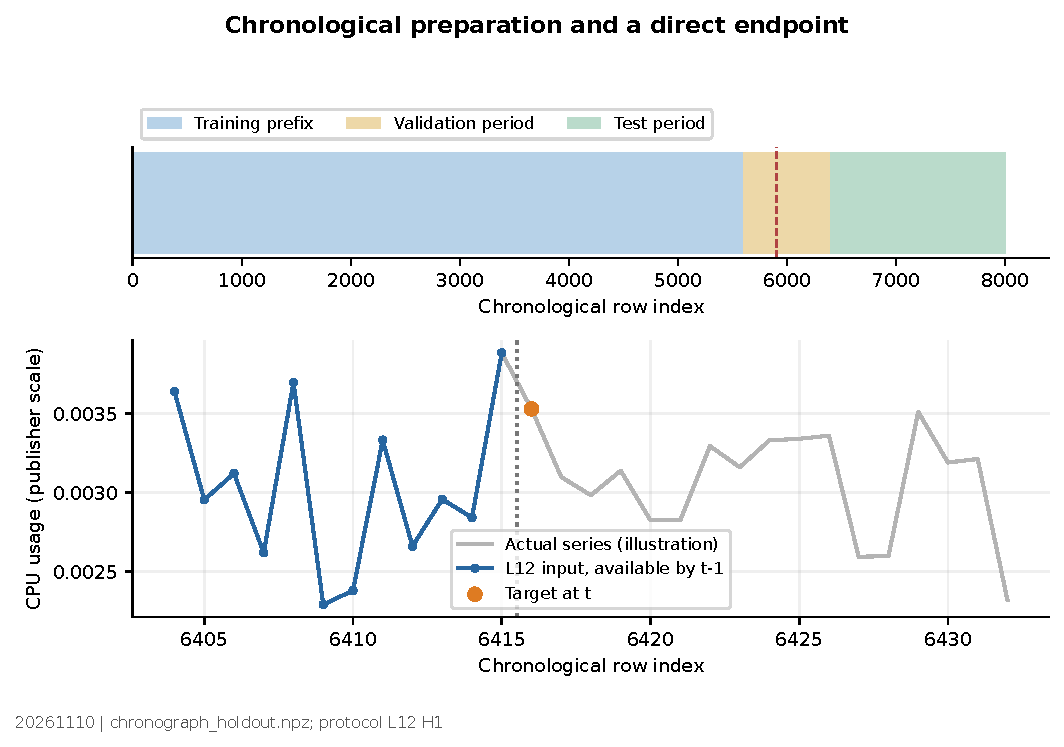
\includegraphics[width=0.72\textwidth]{figuras/04_temporal_preparation.pdf}
\caption{Row-based chronological preparation. The gap after row 5907 belongs to validation. The lower panel uses actual service values to illustrate an L12/H1 input; grey later values are displayed for context and are excluded from the forecast input.}\label{fig:temporal}\end{figure*}

\begin{figure*}[t]\centering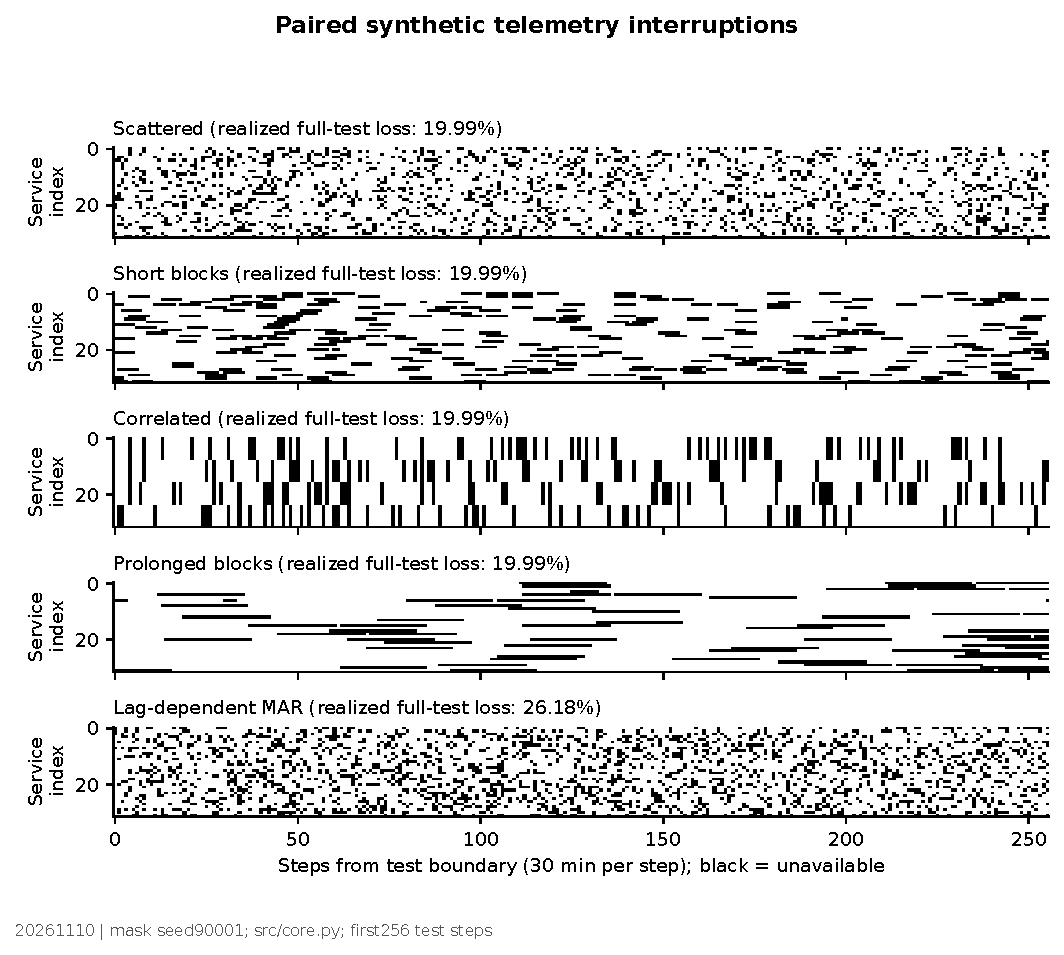
\includegraphics[width=0.68\textwidth]{figuras/05_missingness.pdf}
\caption{Actual masks generated from seed 90001, showing the first 256 test steps. Black indicates unavailability. Correlated groups and block duration are imposed mechanisms. Lag-MAR's probability varies and is not an exact 20\% loss condition.}\label{fig:masks}\end{figure*}

\subsection{Fixed decomposition and compact availability descriptors}
For a filled window $v\in\mathbb{R}^{L}$ and a fixed linear smoothing matrix $S$, DLinear is
\begin{align}
 \widehat x&=w_t^\top Sv+w_r^\top(I-S)v+b_t+b_r\nonumber\\
 &=\underbrace{[S^\top w_t+(I-S)^\top w_r]}_{w_{\rm eff}}^\top v+\underbrace{b_t+b_r}_{b_{\rm eff}}.
\end{align}
The implementation uses a fixed MA25 with replicated padding, including when $L=12$. The centered filter uses only the already available input window; it does not access future forecast targets. Its residual is not established to be a seasonal component. The two-head and collapsed forms define the same affine function class, but Adam and weight decay need not follow equivalent trajectories in the two parameterizations.

A0 uses $w_{\rm eff},b_{\rm eff}$ as a single affine head. A1 adds the window missing fraction $u=L^{-1}\sum_i(1-m_i)$; A2 adds the final log-age $a=\log(1+\delta_{\rm last})/\log(1+L)$; and A3 adds both:
\begin{equation}
 \widehat x_{\mathrm{A3}}=w^\top v+b+\gamma u+\eta a.
\end{equation}
The A0--A3 value function is initialized from the same seeded DLinear heads; additional coefficients start at zero. Float32 initialization equivalence is checked with relative tolerance $10^{-5}$ and absolute tolerance $10^{-6}$, not bitwise equality. The log-age is not clipped in A2/A3. Their parameter counts are $L+1,L+2,L+2,L+3$, versus $2L+2$ for DLinear. The proposal is a parameterization and descriptor study, not a new linear function class. Each family is independently tuned, so these comparisons do not isolate descriptor effects at identical selected hyperparameters.

E5 preserves the historically chosen availability-dependent EMA coefficient $\alpha=0.7$, observation, carry and fallback descriptors and a linearly capped age channel. It has $6L+2$ parameters. Its mask-dependent decomposition is not the fixed $S$ used in the algebraic collapse above. A3 is therefore not an exact collapse of E5. Figs.~\ref{fig:dlinear} and~\ref{fig:a3} show these model distinctions.

\begin{figure*}[!t]\centering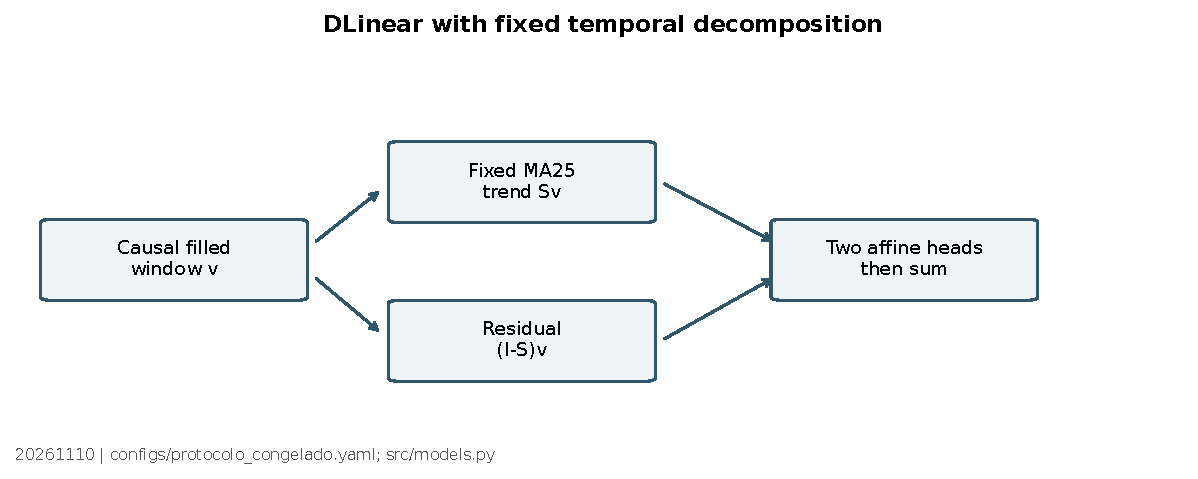
\includegraphics[width=0.79\textwidth]{figuras/02_dlinear.pdf}
\caption{Fixed DLinear decomposition. Both filtered components depend only on the available past window. A fixed smoothing matrix permits algebraic collapse to an affine head, without guaranteeing an identical optimizer trajectory.}\label{fig:dlinear}\end{figure*}

\begin{figure*}[!t]\centering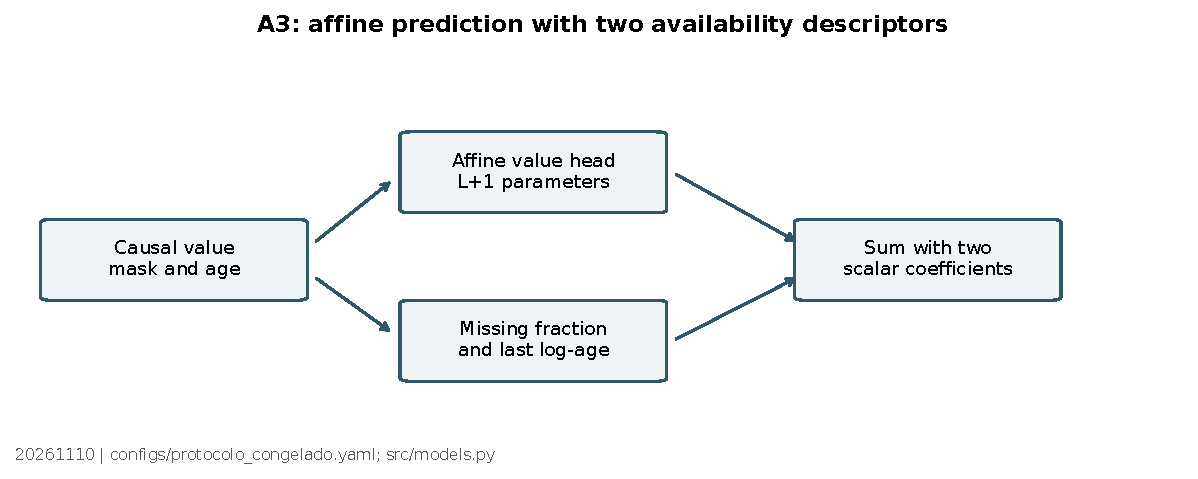
\includegraphics[width=0.79\textwidth]{figuras/03_a3.pdf}
\caption{A3 adds missing fraction and last log-age to the collapsed affine value head. With L12 it uses 15 trainable parameters per resource. Extra coefficients start at zero; descriptor families are tuned independently.}\label{fig:a3}\end{figure*}

\subsection{Historical decomposition, compact families and selection}
The original E0 is fixed MA25 DLinear with 26 trainable parameters per resource. E1 selects a moving-average width from 3, 7, 13 and 25. E2 replaces its level with an observation-updated exponential component. For prepared value $v_i$, indicator $m_i$ and initial level $\ell_1=v_1$, the recurrence is
\begin{equation}
\ell_i=\ell_{i-1}+\alpha m_i(v_i-\ell_{i-1}),\qquad r_i=v_i-\ell_i.
\end{equation}
The historical search considered fixed $\alpha=0.1,0.3,0.7$ and a sigmoid-constrained learned scalar; the selected final configurations use fixed factors. E3 adds a bias-free projection of the 36 availability/carry/fallback indicators, E4 adds a bias-free projection of twelve ages, and E5 combines the exponential component with both heads. Thus E3, E4 and fixed-factor E5 contain 62, 38 and 74 parameters. The added heads start at zero. Because the three status indicators sum to one and positive age also reveals absence, the ablations do not identify orthogonal causal information effects.

The C families retain the two-head decomposition. They add at most a missing-fraction coefficient and a final-age coefficient:
\begin{equation}
\widehat x_C=\widehat x_{\rm base}+\gamma_p L^{-1}\sum_i(1-m_i)+\gamma_a a_L.
\end{equation}
C0 includes neither coefficient, C1 only missing fraction, C2 only age, and C3 both; parameter counts are 26, 27, 27 and 28. Each selects among MA25, EMA0.3 and EMA0.7. These families differ from A0--A3: the A families collapse the fixed DLinear value heads and contain 13--15 parameters at L12, whereas the C families preserve 26 base parameters. Fig.~\ref{fig:evolution} summarizes this progression. A3 is neither the validation alias V2 nor a simple relabeling of C3.

Historical training uses Adam, learning-rate candidates 0.001/0.003, normalized MSE, gradient clipping at one, batch16, up to twenty epochs and patience five. A rotating condition assignment is modulo seven. The short historical search uses three epochs, 512 training origins and 32 validation origins, with selection details that differ across the original variants. C0--C3 use a common six-candidate decomposition/rate grid per resource: 48 short fits followed by 24 final fits across both resources and three seeds. V2 selects one family per resource using the mean best validation MASE of the three seeded fits, breaking ties by parameter count and family identifier. It reuses that family's weights and predictions. No service-specific or test-time oracle selects V2 outputs.

For L12/H1, the historical valid-origin counts are 5591 training, 777 validation and 1589 test. Origin eligibility respects both the row partitions and the actual time gap. Twenty paired realizations cover seven original conditions. Historical uncertainty uses 10000 resamples of whole mask realizations, seed91001, and a crossed three-seed/twenty-mask sensitivity. The historical percentage reduction is calculated after averaging within each mask realization. The expanded percentage estimand instead averages paired service-level cell percentages. These definitions are retained rather than equated merely because both are called reductions.


\subsection{Comparator implementations}
The simple references are persistence, moving average, exponential smoothing and ridge regression with an intercept. Moving-average candidates are 1, 3, 6 and 12 steps, even for longer input windows. Exponential smoothing uses $\alpha\in\{0.1,0.3,0.7,0.9\}$ and updates only on available measurements. Ridge uses $\lambda\in\{0,10^{-4},10^{-2},1\}$, with the intercept unpenalized, fitting all ten prepared training conditions analytically. DLinear, NLinear and the A/E families share their weights across services and predict one resource at a time.

The GRU variants use hidden width 12 and nine input channels per step. GRU (own) repeats the local value/mask/age triplet in three slots to match the graph model's input width. GRU (graph) replaces two slots with incoming and outgoing row-normalized graph aggregates; it contains 841 trainable parameters, as does the width-matched local comparator. The GRU-D adaptation has 615 parameters, decays the input toward normalized mean zero, decays its hidden state and uses a GRU cell with value/mask inputs. This shared-service adaptation is not the canonical clinical multivariate experiment.

PatchTST uses the official Apache-2.0 code at commit \texttt{204c21efe0b3} (full identifier in the code manifest): one input channel, patch length 4, stride 2, end padding, one layer, model width 16, two heads, feed-forward width 32, dropout 0.1 and affine RevIN. The output is the single direct endpoint. At L12 it has 2499 trainable elements plus one fixed attention-scale element registered as a non-trainable parameter. Frozen checkpoint metadata counting all parameter tensors is preserved, while reported trainable counts filter \texttt{requires\_grad}. Calibration, graph buffers, optimizer states and input caches are outside the trainable-count definition. This compact recipe does not reproduce PatchTST's published benchmark settings. TimesNet, iTransformer, TimeMixer and TiDE are not executed in the new queue; historical BiTGraph and GinAR results remain visible separately.

\subsection{Prediction maps and recurrent inputs}
For prepared history $v$, the persistence prediction is $v_L$. Moving average uses $k^{-1}\sum_{i=L-k+1}^L v_i$, and simple exponential smoothing uses the last state of the availability-updated recurrence above. Ridge minimizes $\sum_j(x_j-w^\top v_j-b)^2+\lambda\|w\|_2^2$ over prepared source examples $j$. NLinear predicts $v_L+w^\top(v-v_L\mathbf1)+b$. These expressions are in normalized units, with the same inverse transformation applied before scoring. Their simplicity gives a direct check on how much signal a richer input representation must add to justify its cost.

Let $q_i$ contain value, observation indicator and age for each service at step $i$. The graph GRU consumes the concatenation $[q_i,D_{\rm out}^{-1}Gq_i,D_{\rm in}^{-1}G^\top q_i]$, with zero rows for absent neighbors. The local model uses identity matrices in both aggregate slots. The recurrent map is $h_i=\operatorname{GRU}(u_i,h_{i-1})$, with final affine head $w^\top h_L+b$. For GRU-D, decay vectors are $g_x=\exp[-\operatorname{ReLU}(W_x\delta+b_x)]$ and $g_h=\exp[-\operatorname{ReLU}(W_h\delta+b_h)]$. The cell receives $[m_iv_i+(1-m_i)g_xv_i,m_i]$ and previous state $g_h\odot h_{i-1}$, initialized at zero. This is a decay of the prepared value toward normalized zero, not an inference of the hidden measurement. The dynamic neighbor buffers and their chronology are distinct from model parameters.

PatchTST applies reversible instance normalization \cite{revin}, projects strided length-four patches with positional information, and maps the encoded patches to one target. Within each attention head the encoder applies $\operatorname{softmax}(QK^\top/\sqrt{d_k})V$ to patch embeddings. The final head and inverse normalization return the endpoint to the prepared input scale. This description concerns the executed one-channel recipe. The historical BiTGraph and GinAR retain their archived author-code adaptations and finite-validation guards. Their results are provenance records for the corresponding local implementation rather than estimates for a new implementation of those published methods.

One practical difference between the learned comparators is what happens when a window contains no newly observed values. The last prepared input, its mean and the recursive level can all be defined from causal carry or fallback. Descriptor-aware models can also react to the provenance and age channels. Such cases contribute to the same paired evaluation as more densely observed histories. The pipeline preserves their original targets and does not remove large errors selectively. This supports comparison of conditional point forecasting performance under the implemented masks, while leaving real outage detection and recovery outside the design.

\subsection{Selection, fitting and frozen evaluations}
Every neural family/resource/setting receives four source-only candidates: learning rate $\{0.001,0.003\}$ crossed with weight decay $\{0,0.001\}$. Candidate training uses three epochs, 512 training origins and 64 validation origins, with selection by third-epoch validation MASE over all ten conditions. The search seed is 101. Final fits use the full source training origins, Adam, normalized MSE, gradient clipping at 1, at most 20 epochs, patience five and the best source-validation checkpoint. Each origin receives one rotating condition per epoch, indexed by $(\mathrm{position}+\mathrm{epoch})\bmod10$, rather than ten complete copies per epoch. Source validation and target evaluation use all conditions. Equal candidate counts are not equal FLOPs or equal elapsed search time; ridge's all-condition analytic fit is another explicit budget difference.

Primary L12/H1 neural seeds are 101, 202, 303, 404, 505, 606, 707, 808, 909 and 1010. These represent ten fits conditional on the fixed selected configurations, not ten datasets. Four neural families---DLinear, E5, A3 and PatchTST---and the four simple references form a secondary star design: $(L,h)=(12,2),(12,4),(12,6),(12,12),(24,1),(48,1)$. It uses the first three training seeds and five masks. Horizons are 30, 60, 120, 180 and 360 minutes at L12; histories are 12, 24 and 48 half-hour steps at H1. This is not a complete history-by-horizon factorial. For secondary curves, all seven settings are recomputed over the same intersection of valid target rows and matching three-seed/five-mask subset. The full primary endpoint remains unchanged.

The protocol and training sources are hashed locally before primary target evaluation. Each setting freezes all families and both resources before evaluating that setting. Secondary source-only selections occur later in the automated queue; target errors are not used for retuning. Two pretest amendments accelerated GRU-D through numerically verified CUDA Graph replay and removed a per-stream CUDA workspace accumulation. Candidate source-validation selections remained unchanged. Seven GRU-D source fits initially failed with memory errors and were retried under the recorded amendment; no model was dropped based on test performance. One retained primary GRU-D CPU-resource fit used microbatch 4 after the prescribed reduction. Checkpoints retain completed-epoch optimizer, RNG and sampler states; simulated interruption tests check exact same-backend resumption.

\begin{table*}[!t]
\caption{Master design. H denotes minutes and L half-hour steps. Simple models have one fitted or selected record rather than artificial neural-seed replication. No cross-cohort pooled endpoint is constructed.}\label{tab:master}
\centering\footnotesize
\begin{tabularx}{\linewidth}{p{.15\linewidth}p{.17\linewidth}p{.23\linewidth}X}
\toprule Phase & Cohort & Replication and settings & Role and metrics \\\midrule
I & Source28 & E0--E5 and original references; 3 seeds/20 masks; L12/H30 & Historical exploratory; MAE/RMSE/MASE and paired reductions \\
II & Source28 & C0--C3; V2 alias; 3/20; L12/H30 & Validation selection; conditional/crossed uncertainty \\
III & Destination32 & 15 families; 10 neural seeds/20 masks; L12/H30 & Four prespecified contrasts; complete/stress conditions secondary \\
IV & Destination32 & Eight families; 3 neural seeds/5 masks; six extensions & Direct H60/120/180/360 or L24/48; common-support MASE \\
IV & Alibaba32 & 14 eligible families; frozen source fits; 20 masks & 12 calibration bins,36 targets; normalized absolute errors/MASE \\
V & Source28 and destination32 & Historical B128 CUDA and new B1/B128 CPU/CUDA & Parameters, p50/p95, epoch times, RSS and allocation; separate protocols \\
\bottomrule
\end{tabularx}
\end{table*}

\subsection{Formal error and cost definitions}
For a valid service/resource series with $T$ targets, define
\begin{align}
\operatorname{MAE}&=T^{-1}\sum_t|\widehat y_t-y_t|,\notag\\
\operatorname{RMSE}&=\sqrt{T^{-1}\sum_t(\widehat y_t-y_t)^2},\\
d_{s,r}&=|P|^{-1}\sum_{t\in P}|y_{t,s,r}-y_{t-1,s,r}|,\notag\\
\operatorname{MASE}&=\operatorname{MAE}/d_{s,r}.
\end{align}
$P$ contains available adjacent training-prefix pairs separated by 1800 seconds. MAE and RMSE retain the target's units; MASE is dimensionless. A test persistence forecast need not have MASE one, since its errors and the training denominator come from different periods. Averaging service RMSE values is not equivalent to taking one square root after pooling every squared residual. Equal service weighting also differs from weighting services by resource magnitude or request traffic.

For paired errors $e_B,e_M$, $\Delta=e_B-e_M$ and $R=100(e_B-e_M)/e_B$ favor $M$ when positive. The aggregation level used to form $R$ is explicitly reported. Model size counts trainable scalar elements. A latency percentile is an empirical quantile of timed calls on a specified device and batch; throughput additionally depends on how many origins and services the call includes. Training duration includes completed optimization epochs and validation under the recorded timing scope. Neither parameter count nor forward latency measures total energy or monetary cost.


\subsection{Pairing and statistical interpretation}
For each service, we compute MAE and RMSE over valid target times in physical or publisher-normalized units. MASE divides MAE by the mean absolute one-step difference in that service's training prefix \cite{mase}, excluding time gaps and unavailable consecutive values. A zero denominator produces an undefined MASE, not an artificial constant; the observed denominators are all positive. Macro RMSE averages service-level square roots, not a pooled root mean square. The primary endpoint averages equally over services, the six original positive-loss conditions, twenty mask realizations and the seeded fits. The complete and three added conditions remain secondary.

For reference $B$, define $\Delta=\mathrm{MASE}_{B}-\mathrm{MASE}_{A3}$, with positive values favoring A3. We retain per-cell paired percentage reductions $100(e_B-e_{A3})/e_B$, excluding zero-reference cells only from the percentage calculation. The mean paired percentage is distinguished from a percentage calculated using the ratio of aggregate means. The absolute effect does not require either percentage definition.

Four exact two-sided sign tests use the ten seed-mean paired differences: A3 versus DLinear and E5, for CPU and memory. Ties are excluded and the four tests receive Holm correction \cite{holm}. The sign-test null concerns $\Pr(\Delta_{\rm seed}>0)=1/2$ under the conditional seeded-run model; it is not a general test that the arithmetic mean difference is zero. Seed 101 also appears in source tuning. A pre-target-inspection sensitivity removes this seed, reports nine-seed effects and separately adjusted diagnostic sign tests; it does not replace the primary analysis.

Uncertainty intervals use 2000 crossed bootstrap replicates of seed indices, mask indices and circular temporal blocks, with bootstrap seed 61110. Services stay together rather than being resampled as independent infrastructures. The main block length is 48 steps, with 24/96-step sensitivity. Intervals are conditional on this trace, these fixed services and the selected configurations; temporal stationarity and finite-sample bootstrap limitations remain. They are neither population-level infrastructure intervals nor prediction intervals. Per-service effects, seed/mask standard deviations and non-overlapping 48-origin descriptive period summaries accompany aggregate estimates. Secondary and external comparisons do not receive confirmatory significance claims.

\subsection{Hardware, execution and measurement}
Execution uses Docker with Debian GNU/Linux 13, Python 3.12 and PyTorch 2.9.0+cu128 on an Intel Core i5-11300H (4 cores/8 threads), approximately 24 GB RAM and NVIDIA RTX 3050 Laptop GPU (4 GB nominal VRAM), driver 550.163.01. GPU training uses float32, two CPU threads, an effective batch of 16 and microbatch 8 with accumulation. PatchTST BatchNorm sees the microbatch, not a physical batch of 16. Deterministic algorithms are enabled and TF32 disabled. A single project GPU queue coexists with other user applications; project monitors sample memory, temperature and swap activity and can pause only the project runner. Drivers, security settings and other services are unchanged.

After training, CPU and CUDA inference are benchmarked sequentially at batches 1 and 128, each with 32 services, on resident tensors. Twenty warmups precede 100 timed trials per model/device/batch, with CUDA synchronization and a fixed randomized model order. The reported p50/p95 and throughput exclude data acquisition, preprocessing, transport and orchestration. GRU-D eager and CUDA replay measurements are separate; replay latency excludes initial graph capture. Completed-epoch sums include validation and initial capture but exclude checkpoint I/O, search and incomplete failed attempts. Shared-laptop timing, including earlier fits concurrent with data preparation, cannot identify architecture-only training-cost effects. Process RSS and PyTorch allocation have distinct scopes; whole-system VRAM cannot be attributed to this project. No reliable energy instrument was available, so no energy claim is made.





\section{Results}
\subsection{Historical reconstruction and original model comparison}\label{sec:historical-loss}
The historical audit preserved original results and checked 1720 physical prediction files: 1240 earlier files by integrity checks and 480 compact-model files through recomputation. The 337120 physical metric rows exclude the extra 23520 V2-labeled alias rows. In the reproduced original comparison, thirty trained final states matched the archived reference states; an aggregate MASE discrepancy of $4.66\times10^{-10}$ was retained as numerical summary precision rather than interpreted as retraining improvement. Earlier pilot documents included a different partition, but the analysis here uses the actually executed 70/10/20 version.

Table~\ref{tab:historical-main} reports the six positive-loss conditions for the 28-service cohort. E5 has CPU MASE1.002387 versus E0's 0.992620, and memory MASE1.121358 versus 1.135901. Its mask-paired percentage changes are therefore unfavorable for CPU ($-0.984\%$ reduction) and favorable for memory ($1.280\%$). GRU with calls has the lowest displayed historical CPU MASE, 0.939410; this local result does not establish general graph superiority. Historical GinAR CPU MASE is 280825.103210, an extreme retained result of this implementation and budget. Verification did not justify discarding it or equating it with the published method's expected behavior.

\begin{table*}[!t]
\caption{Historical six-positive-loss means, source28, three neural seeds and twenty masks. Absolute CPU errors retain publisher scale and memory errors are bytes. V2 is a selected alias, not an additional fit. These values must not be mixed with destination32 errors.}\label{tab:historical-main}
\centering\footnotesize
\FitTable{\begin{tabular}{lrrrrrr}
\toprule
Model & CPU MASE & CPU MAE & CPU RMSE & Mem. MASE & Mem. MAE & Mem. RMSE \\
\midrule
persistencia & 1.07741 & 0.000300957 & 0.000505471 & 1.31287 & 1.30725e+06 & 2.01898e+06 \\
E0 & 0.99262 & 0.000302127 & 0.000456189 & 1.1359 & 1.10867e+06 & 1.694e+06 \\
E1 & 1.02275 & 0.000307441 & 0.000457202 & 1.1359 & 1.10867e+06 & 1.694e+06 \\
E2 & 1.02163 & 0.000305333 & 0.000453692 & 1.12503 & 1.09644e+06 & 1.6773e+06 \\
E3 & 1.00514 & 0.000304111 & 0.000455915 & 1.1345 & 1.10712e+06 & 1.69482e+06 \\
E4 & 0.98954 & 0.000301872 & 0.000456377 & 1.13528 & 1.10705e+06 & 1.69286e+06 \\
E5 & 1.00239 & 0.000305151 & 0.000455849 & 1.12136 & 1.0933e+06 & 1.67625e+06 \\
C0 & 1.02163 & 0.000305333 & 0.000453692 & 1.1359 & 1.10867e+06 & 1.694e+06 \\
C1 & 1.02095 & 0.000305271 & 0.000453709 & 1.1351 & 1.10785e+06 & 1.69341e+06 \\
C2 & 1.02151 & 0.000305326 & 0.000453707 & 1.13576 & 1.10848e+06 & 1.69381e+06 \\
C3 & 1.02092 & 0.000305271 & 0.000453723 & 1.13522 & 1.10794e+06 & 1.69342e+06 \\
V2 & 1.02092 & 0.000305271 & 0.000453723 & 1.1351 & 1.10785e+06 & 1.69341e+06 \\
GRU\_propia & 0.955358 & 0.000279717 & 0.0004371 & 1.16785 & 1.15154e+06 & 1.76786e+06 \\
GRU\_llamadas & 0.93941 & 0.000274958 & 0.000430716 & 1.19984 & 1.18269e+06 & 1.81389e+06 \\
BiTGraph\_codigo\_autor & 1.00373 & 0.000282931 & 0.000428389 & 1.21558 & 1.18535e+06 & 1.79317e+06 \\
GinAR & 280825 & 63.2538 & 1254.57 & 2.5045 & 2.27786e+06 & 4.49626e+06 \\
\bottomrule
\end{tabular}}
\end{table*}

Within E0--E5, E2's exponential component improves mean memory MASE to 1.125032 but worsens CPU to 1.021630. E4 gives the lowest CPU MASE among these six variants, 0.989540, while its memory MASE is 1.135284. E1 and E3 do not produce simultaneous resource gains. E5's combination is thus not a monotonic accumulation of improvements. The added memory benefit relative to E2 is a paired reduction of approximately 0.327\%, with more parameters and measured inference cost. These are independently selected configurations, so component names do not by themselves identify causal contributions.

\subsection{Compact C families, V2 and historical uncertainty}\label{sec:historical-compact}
C0--C3 reduce descriptor dimensionality without collapsing the two value heads. Their historical CPU MASE values are 1.021630, 1.020946, 1.021505 and 1.020919; memory values are 1.135901, 1.135097, 1.135755 and 1.135218. V2 selects C3/EMA0.7 for CPU and C1/MA25 for memory, with mean validation MASE0.911214 and 0.998329, respectively. The resulting test MASE is 1.020919/1.135097, with paired reductions of $-2.851\%$/$0.071\%$ against E0. Against E5 the reductions are $-1.849\%$/$-1.225\%$. Compactness therefore did not preserve E5's historical memory gain or improve both resources over E0.

The narrow mask-only E5 difference intervals are $[-0.010137,\allowbreak -0.009395]$ for CPU and $[0.014296,\allowbreak 0.014793]$ for memory. Crossing seed and mask resampling widens the CPU interval to $[-0.028165,\allowbreak 0.026164]$. The corresponding memory interval is $[-0.002967,\allowbreak 0.024027]$. Both include zero. One of three seed means favors E5 on CPU and two of three on memory. Although all 28 memory service means favor E5 after averaging other factors, those services are connected and share the same trace; this is not a binomial sample of infrastructures. Historical uncertainty therefore supports an observed memory advantage conditional on fits, with substantial initialization sensitivity.

Fig.~\ref{fig:historical} puts the historical rank and the extreme GinAR result on readable resource-specific axes. The historical displayed E0/E2/E4/E5/V2 curves rise across 0,10,20 and40\% loss under both original patterns for both resources. This yields twenty displayed increasing curves, not a theorem over every comparator or individual series. Historical CUDA B128 timing further shows why compression alone is insufficient: CPU-target E0/E5/V2 p50 values are 0.284/0.814/0.691 ms, and memory-target values 0.287/0.801/0.416 ms. V2 uses 28 CPU and27 memory parameters versus E5's74, but CPU V2 remains slower than E0. These ten-warmup eager measurements are not pooled with the later twenty-warmup B1 results.

\begin{figure*}[!t]\centering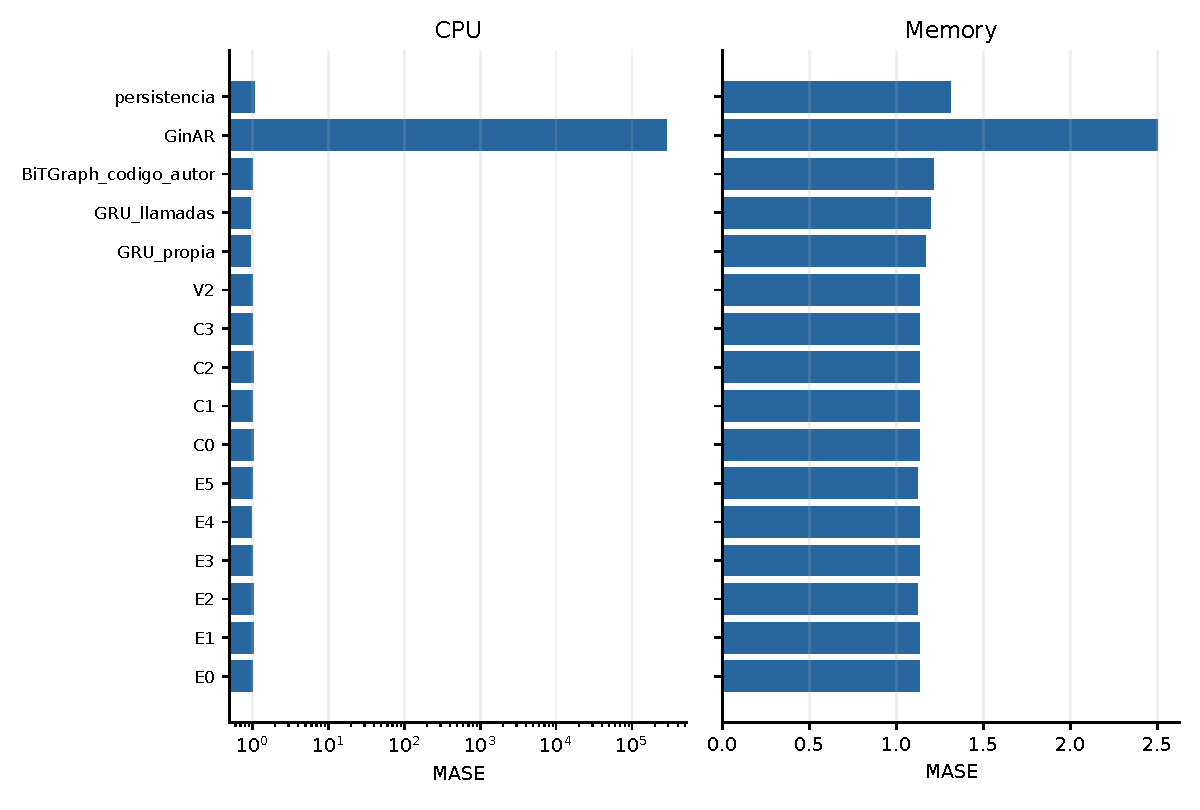
\includegraphics[width=0.82\textwidth]{figuras/historico.pdf}
\caption{Historical MASE under six positive-loss conditions. Logarithmic CPU scale preserves GinAR's extreme local value. Memory uses a linear scale. These are source28 results, not the destination comparison.}\label{fig:historical}
\end{figure*}
\begin{figure*}[!t]\centering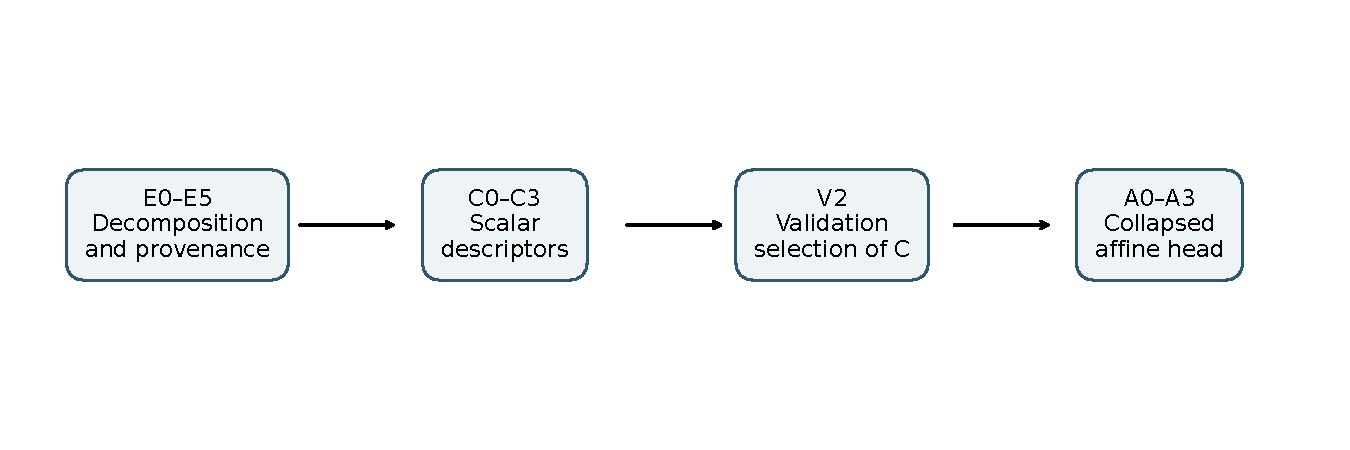
\includegraphics[width=0.91\textwidth]{figuras/evolucion.pdf}
\caption{Experimental progression: E changes decomposition or full descriptors; C retains two value heads with scalar descriptors; V2 selects existing C fits; A collapses the fixed affine value map. Arrows describe study order, not guaranteed accuracy gains.}\label{fig:evolution}
\end{figure*}


\subsection{Completion, integrity and realized loss}\label{sec:completion}
The project completed the L12/H1 primary setting, six secondary settings and the external frozen-weight transfer. It retained 364 final neural fits and 56 simple model/setting/resource records, with 280 short source-only candidate fits. The complete new study contains 9680 saved prediction arrays and 3,097,600 service-level metric rows. An independent float64 reconstruction from all arrays checked target indices and counts, array digests, MAE, RMSE and MASE against the saved CSVs. The largest absolute metric reconstruction difference was $3.73\times10^{-9}$ in physical units. The 420 final checkpoints and frozen-source hashes passed the checkpoint audit. These rows are repeated model/seed/mask/condition/service summaries, not independent data sources.

At nominal 20\% loss, the four exact-count mechanisms produced 19.988\% induced unavailability on the ChronoGraph test segment; lag-MAR averaged 26.301\% across twenty masks, ranging from 25.925\% to 26.577\%. In the 48-bin external case, rounding gives 20.833\% for exact-count mechanisms, while lag-MAR averaged 27.861\% (26.042\%--30.469\%). Natural missingness is recorded separately. Fig.~\ref{fig:masks} makes the imposed spatial and duration structure visible. The 70/10/20 source cut is a row split; the external case has 12 calibration and 36 target bins.

\subsection{Primary 32-service comparison}
Table~\ref{tab:primary} and Fig.~\ref{fig:models} report the prespecified six positive-loss original conditions at L12/H1. PatchTST has the lowest observed mean MASE, 1.0419 for CPU and 1.2170 for memory; NLinear is close at 1.0463 and 1.2197. No confirmatory comparison between those two models was specified. Moving average has CPU MASE1.0678, below DLinear (1.1493), E5 (1.1454) and A3 (1.1602). For memory, A0 is the lowest compact affine variant at 1.2334, whereas A3 is 1.2403, DLinear 1.2402 and E5 1.2656. Thus the two added availability coefficients do not produce an aggregate A3 gain over A0. E5's favorable historical memory result does not carry over as a win over DLinear in this new cohort. The graph GRU's memory MASE is 1.4851; none of the neural families was removed because of an unfavorable score.

\begin{table*}[!t]
\caption{Primary new-service means over equal service, original positive-loss condition, mask and seeded-fit weights. CPU absolute MAE/RMSE are displayed in $10^{-3}$ publisher-scale units; memory absolute errors are in MiB ($2^{20}$ bytes). MASE is dimensionless. Lower is better. No significance is inferred from rank alone.}\label{tab:primary}
\centering\footnotesize
\FitTable{\begin{tabular}{lrrrrrr}
\toprule
Model & CPU MASE & CPU MAE & CPU RMSE & Mem. MASE & Mem. MAE & Mem. RMSE \\
\midrule
Persistence & 1.1170 & 3.3236 & 4.5878 & 1.2861 & 2.0009 & 3.3833 \\
Moving average & 1.0678 & 2.9643 & 4.2038 & 1.2361 & 1.8956 & 3.2699 \\
Exponential smoothing & 1.0691 & 2.8926 & 4.0646 & 1.2535 & 1.9130 & 3.2673 \\
Ridge & 1.2669 & 3.1952 & 4.3079 & 1.3613 & 1.9589 & 3.1848 \\
DLinear & 1.1493 & 2.9924 & 4.1015 & 1.2402 & 1.8762 & 3.1573 \\
NLinear & 1.0463 & 2.8499 & 3.9969 & 1.2197 & 1.8482 & 3.1422 \\
E5 & 1.1454 & 3.0142 & 4.1411 & 1.2656 & 1.9044 & 3.1560 \\
A0 & 1.1562 & 3.0028 & 4.1185 & 1.2334 & 1.8649 & 3.1605 \\
A1 & 1.1547 & 2.9986 & 4.1147 & 1.2397 & 1.8704 & 3.1591 \\
A2 & 1.1563 & 3.0030 & 4.1185 & 1.2443 & 1.8773 & 3.1650 \\
A3 & 1.1602 & 3.0095 & 4.1248 & 1.2403 & 1.8733 & 3.1629 \\
GRU (own) & 1.2198 & 3.2253 & 4.5667 & 1.3438 & 2.1652 & 3.7094 \\
GRU (graph) & 1.1949 & 3.2375 & 4.5153 & 1.4851 & 2.2017 & 3.6563 \\
GRU-D adaptation & 1.1766 & 3.1392 & 4.4427 & 1.3605 & 2.1647 & 3.6811 \\
PatchTST (small) & 1.0419 & 2.8539 & 4.1061 & 1.2170 & 1.8649 & 3.1655 \\
\bottomrule
\end{tabular}
}
\end{table*}

\begin{figure*}[!t]\centering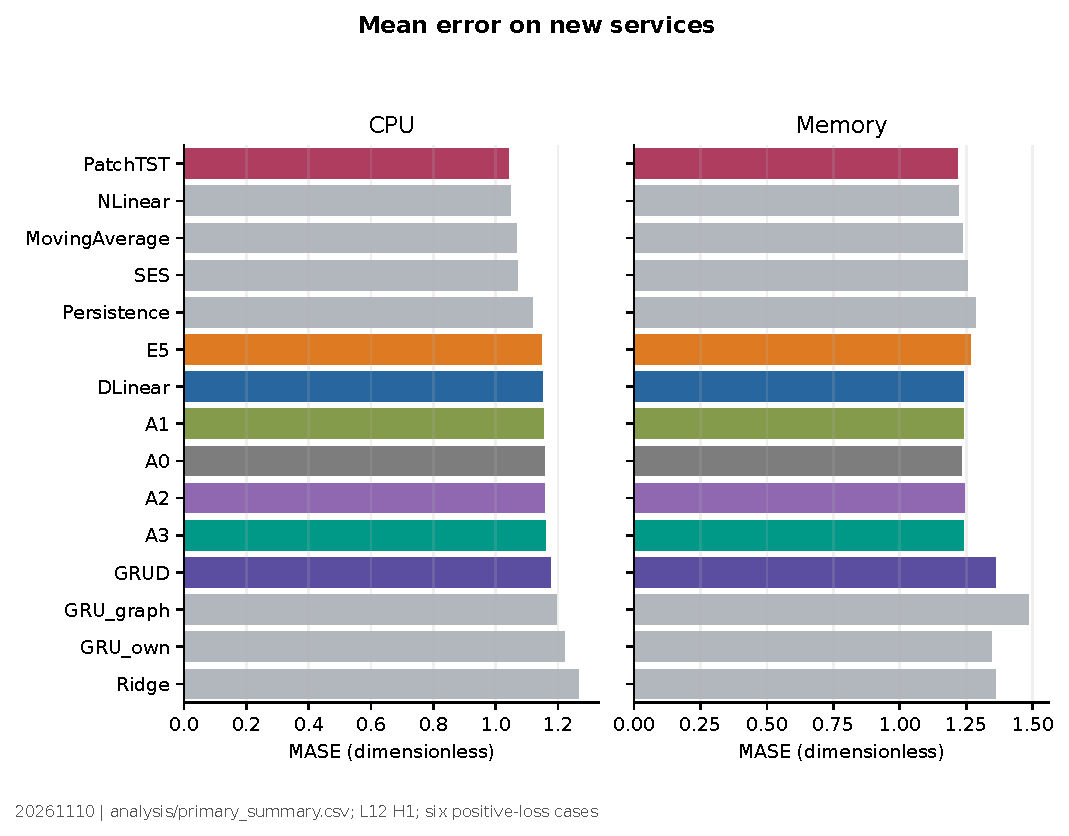
\includegraphics[width=0.79\textwidth]{figuras/06_models.pdf}
\caption{Primary MASE for all 15 newly evaluated families. CPU ordering is only a display choice. Families share the same fixed services, masks and target origins, while neural seed variability remains visible in supplementary material.}\label{fig:models}\end{figure*}


\subsection{Four prespecified paired contrasts}\label{sec:contrasts}
Table~\ref{tab:contrasts} distinguishes a mean MASE difference from a mean per-cell percentage reduction. The sole contrast with ten of ten favorable seed means is A3 versus E5 on memory: $\Delta=0.02523$ MASE, Holm-adjusted exact sign-test $p=0.0078125$, and a conditional 48-step crossed-block 95\% interval $[0.01312,0.03981]$. The mean paired per-cell reduction is 1.00\%; the ratio of aggregate means gives 1.99\%, a different estimand. Excluding the source-tuning seed 101 leaves nine of nine favorable seed means and an exploratory separately adjusted $p=0.015625$. These values concern fixed services, masks and trace and do not establish improvement in a population of cloud systems.

A3 versus DLinear has negative mean $\Delta$ on CPU ($-0.01090$) and nearly zero on memory ($-0.00014$); the adjusted sign-test $p$ is 1 for both. A3 versus E5 on CPU is also negative ($-0.01485$, adjusted $p=1$). Its conditional temporal bootstrap interval excludes zero on the negative side, whereas only three of ten seed means favor A3 and the prespecified sign test is nonsignificant. The two procedures address different sampling assumptions and estimands; the interval does not override the four-test decision rule. Primary block-length sensitivity is listed in Table~\ref{tab:block}.

\begin{table*}[!t]
\caption{Four prespecified A3 contrasts. $\Delta$MASE is reference minus A3; positive values favor A3. Mean $R$ averages paired valid cell percentages, rather than taking a ratio of overall means. Intervals resample seed, mask and time blocks conditional on fixed services; $p$ values are exact two-sided seed-mean sign tests adjusted by Holm.}\label{tab:contrasts}
\centering\footnotesize
\FitTable{\begin{tabular}{lrrrrrr}
\toprule
Resource & Reference & $\Delta$MASE & Mean $R$ (\%) & Conditional 95\% interval & $p_{\mathrm{Holm}}$ & Positive seeds \\
\midrule
CPU & DLinear & -0.01090 & -0.78 & [-0.02732, 0.00470] & 1 & 4/10 \\
CPU & E5 & -0.01485 & -1.95 & [-0.02977, -0.00120] & 1 & 3/10 \\
Memory & DLinear & -0.00014 & 0.00 & [-0.00959, 0.01035] & 1 & 3/10 \\
Memory & E5 & 0.02523 & 1.00 & [0.01312, 0.03981] & 0.007812 & 10/10 \\
\bottomrule
\end{tabular}
}
\end{table*}

The favorable memory mean against E5 is spatially uneven: only 10 of 32 service-level paired mean differences favor A3. Service540 alone contributes 42.4\% of the aggregate mean difference. An outcome-informed \emph{post hoc} sensitivity excluding it still yields a positive mean difference of 0.01499; excluding the three largest favorable services yields 0.00325 and six of ten favorable seed means. These exclusions were chosen after seeing outcomes, so neither resulting sign-test value is confirmatory. Fig.~\ref{fig:services} displays the separately specified DLinear--A3 service differences, which are also heterogeneous. Table~\ref{tab:variation} separates seed and mask variation. Fig.~\ref{fig:seeds} shows the between-fit spread, while Fig.~\ref{fig:ablation} shows that adding both descriptors does not guarantee lower mean error. Masks repeat the evaluation of the same fits.

\begin{figure*}[!t]\centering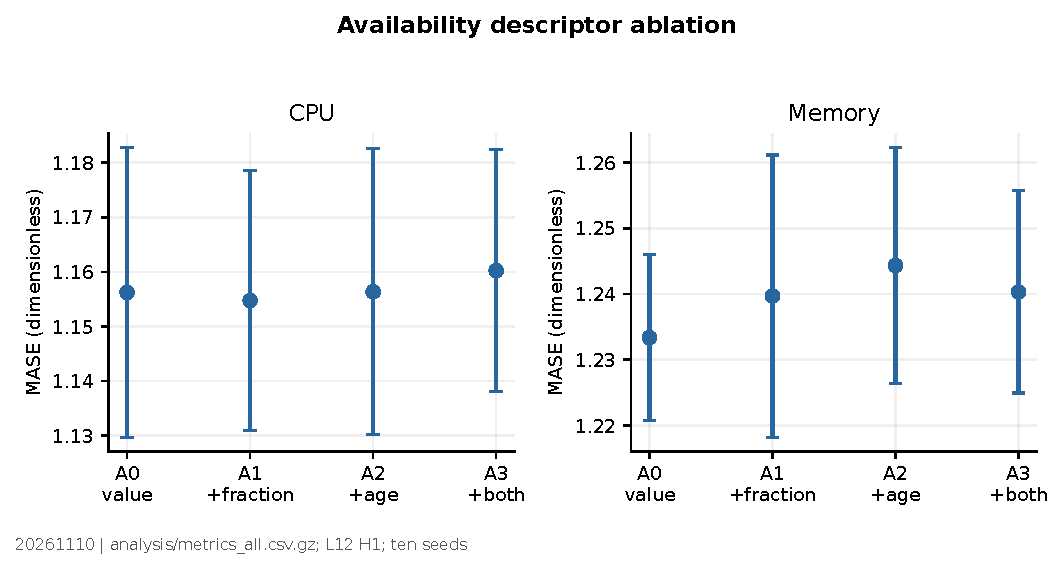
\includegraphics[width=0.79\textwidth]{figuras/11_ablations.pdf}
\caption{A0--A3 means and standard deviations across ten seeded-fit means. Error bars are descriptive standard deviations, not confidence or prediction intervals. Each family was independently tuned on source validation.}\label{fig:ablation}\end{figure*}
\begin{figure*}[!t]\centering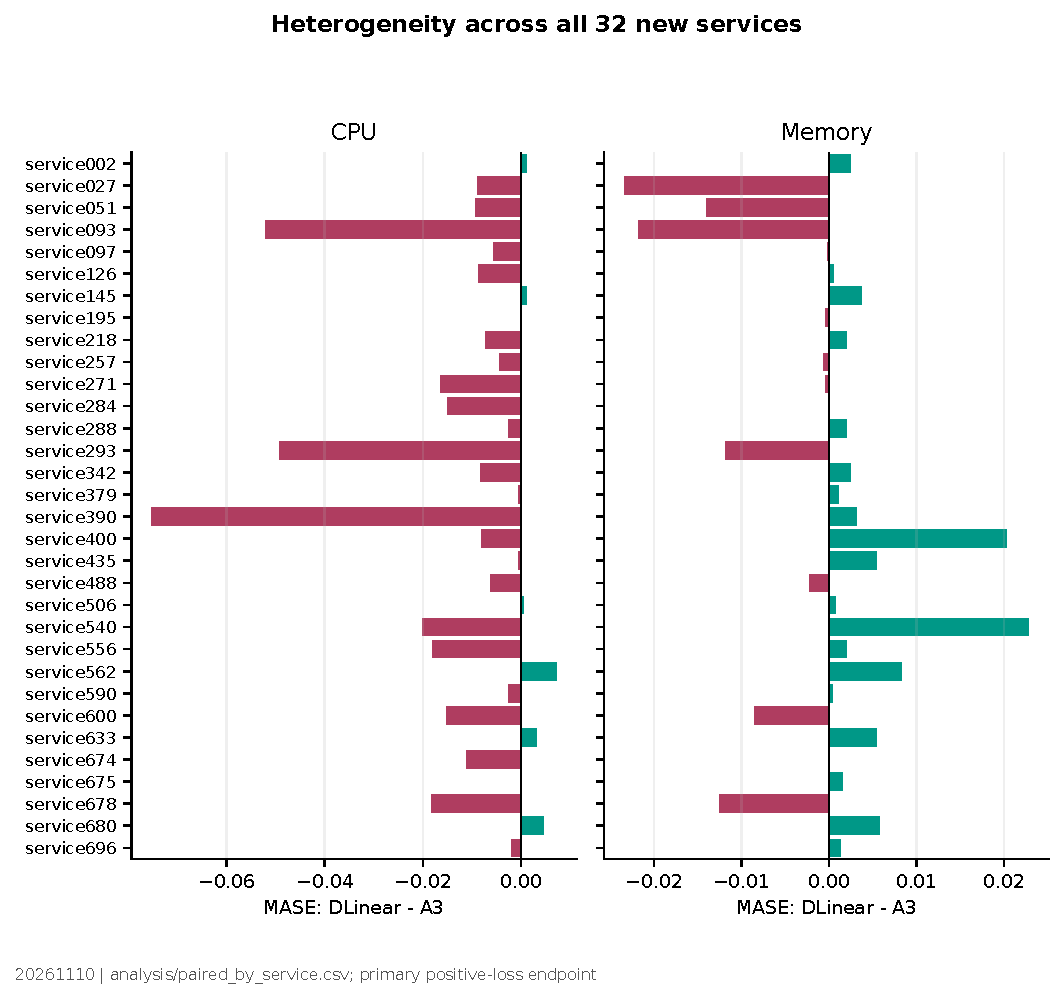
\includegraphics[width=0.71\textwidth]{figuras/15_services.pdf}
\caption{DLinear minus A3 MASE by destination service, averaged over paired seeds, masks and six positive-loss conditions. Positive bars favor A3. These connected services are fixed study cases rather than independent population draws.}\label{fig:services}\end{figure*}

\begin{figure*}[!t]\centering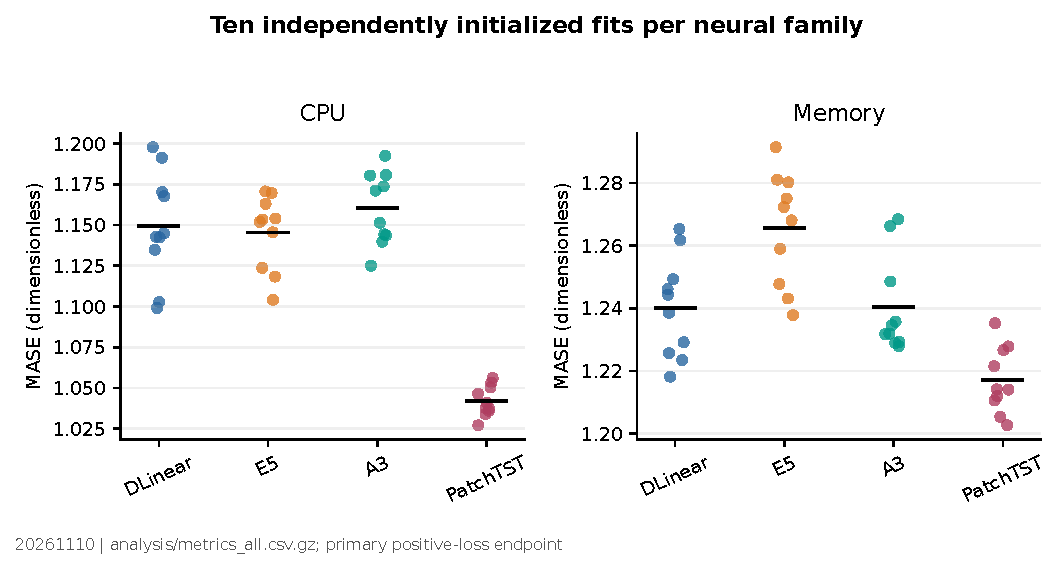
\includegraphics[width=0.76\textwidth]{figuras/10_seed_variability.pdf}
\caption{Ten seeded fit means per displayed neural family, averaged over fixed services, six positive-loss conditions and twenty masks. Black marks denote their mean. These are initialization replicates, not ten infrastructures.}\label{fig:seeds}\end{figure*}
\subsection{Robustness to incomplete telemetry}
Mean error generally rises from complete telemetry to 40\% missingness in the displayed scattered and short-block curves (Fig.~\ref{fig:loss}). This describes model averages, not a monotonicity theorem for every service or mask. At nominal 20\%, prolonged blocks are harder than correlated masks for A3: CPU MASE1.2330 versus 1.1342 and memory 1.3743 versus 1.1932. Lag-MAR is not directly a controlled 20\% comparison because its realized missing fraction is higher. Table~\ref{tab:stress} retains all models and all three added mechanisms; no claim is based on selecting favorable curves alone.

\begin{figure*}[!t]\centering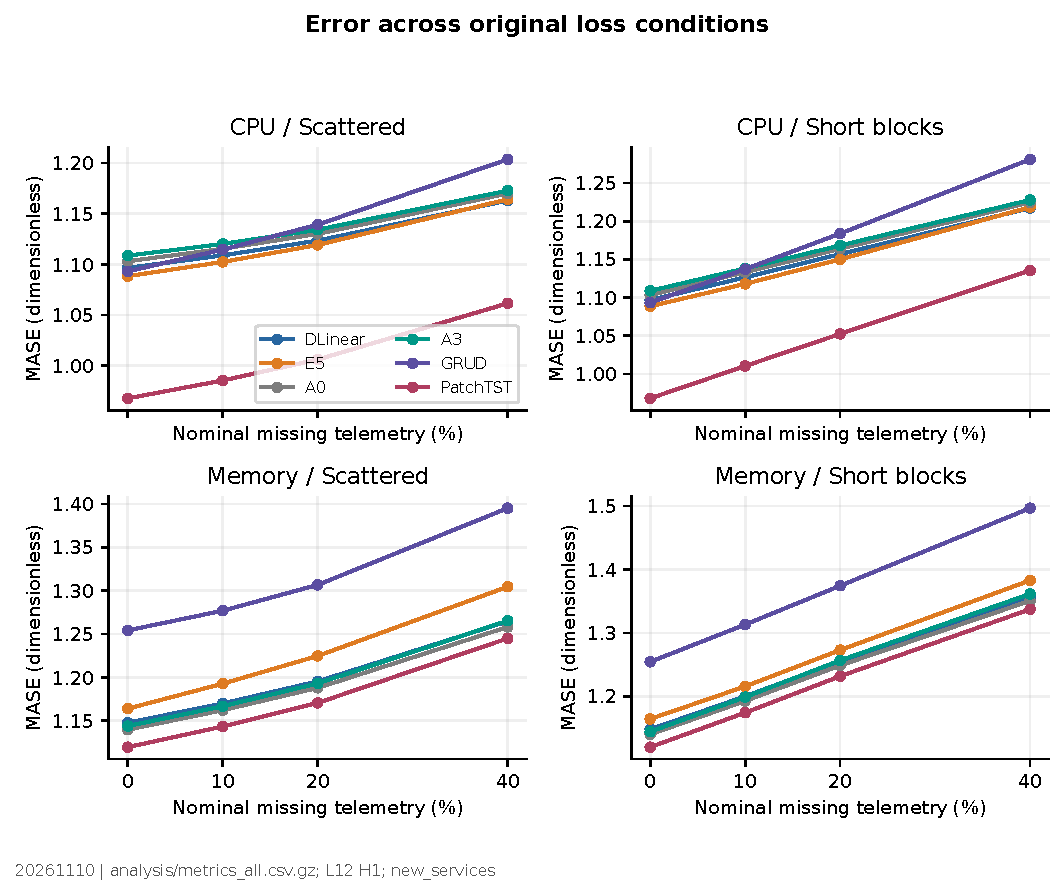
\includegraphics[width=0.76\textwidth]{figuras/07_loss.pdf}
\caption{Descriptive mean MASE under the original complete, scattered and short-block conditions. The six curves shown were chosen for display; Table~\ref{tab:primary} and machine-readable CSVs retain the complete comparison.}\label{fig:loss}\end{figure*}
\subsection{Direct horizons and input histories}
The common-support secondary display uses 1553 identical destination target rows (6452--8004), the first three training seeds, five paired masks and the original six positive-loss conditions. With L12, PatchTST's observed CPU MASE increases from 1.0445 at 30 minutes to 1.6399 at six hours; A3 increases from 1.1584 to 1.9779. Memory increases from 1.2264 to 2.1681 for PatchTST and from 1.2436 to 2.3141 for A3. Each horizon has a separately fitted direct model; these are not iterated one-step predictions. Longer histories at 30 minutes are mixed: A3 CPU improves from 1.1584 (L12) to 1.0966 (L48), while its memory MASE rises from 1.2436 to 1.2560. PatchTST memory is lowest at L24 (1.2190) among its three displayed history lengths. The common-support H30 point deliberately differs from the full primary endpoint and is not a replacement test. Figs.~\ref{fig:horizon} and~\ref{fig:history} and Tables~\ref{tab:horizon}--\ref{tab:history} retain the star-design comparisons.
\begin{figure*}[!t]\centering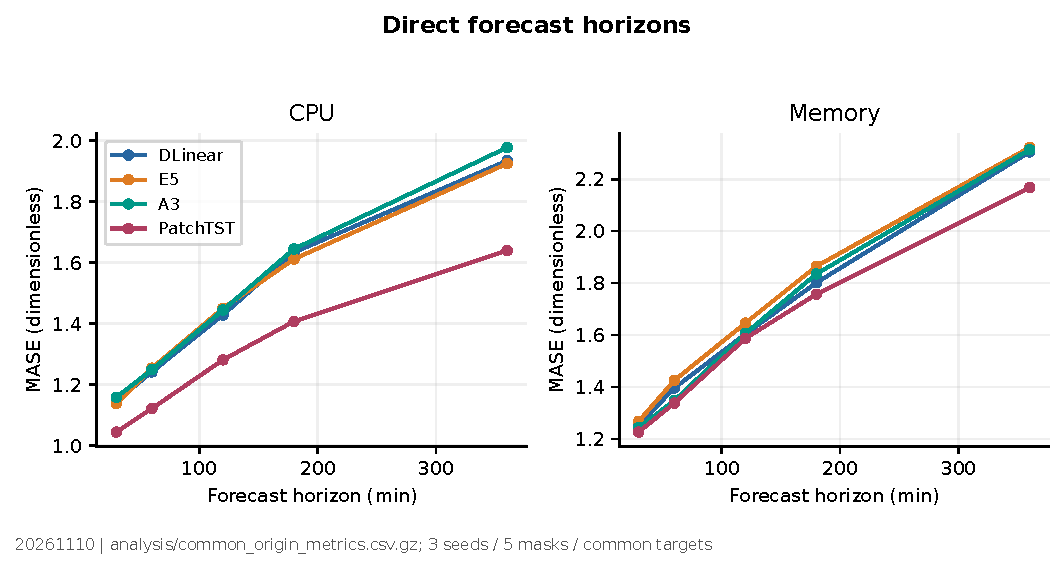
\includegraphics[width=0.79\textwidth]{figuras/08_horizon.pdf}
\caption{Common-target-origin direct-horizon MASE, three seeds and five masks. Each endpoint is fitted directly, using the same fixed 1553 target rows for display; no complete factorial is implied.}\label{fig:horizon}\end{figure*}
\begin{figure*}[!t]\centering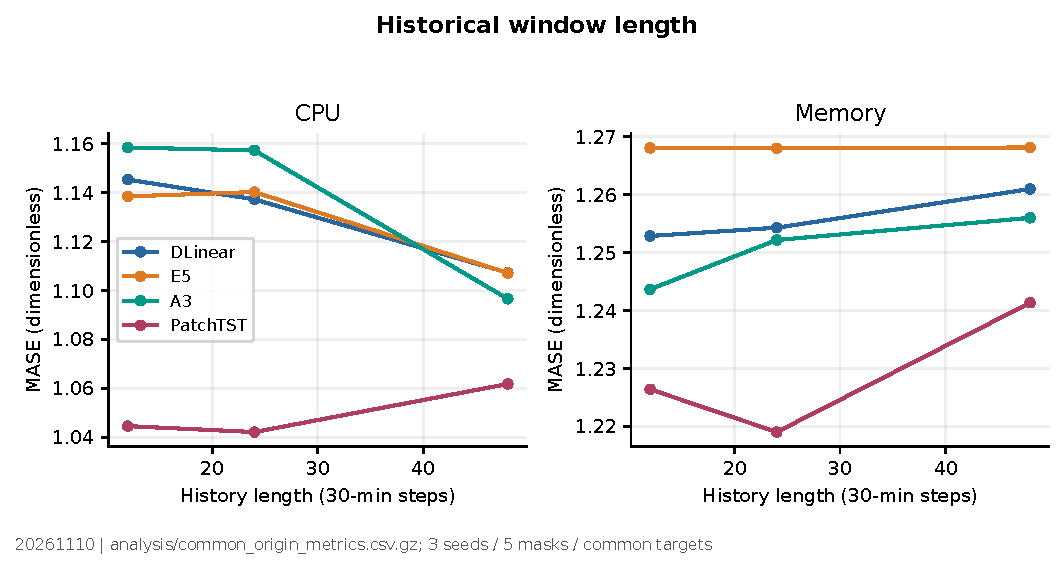
\includegraphics[width=0.79\textwidth]{figuras/09_history.pdf}
\caption{Common-target-origin history sensitivity at a 30-minute horizon, with the same three-seed/five-mask subset. Lines are descriptive and have no confirmatory significance tests.}\label{fig:history}\end{figure*}

\subsection{External transfer and computational cost}\label{sec:cost}
Fig.~\ref{fig:external} shows the external ranking. In the Alibaba day, persistence gives the lowest observed MASE of the 14 eligible families for both normalized CPU (2.3795) and normalized memory (7.5150). A3 is 3.3593 and 9.9535; PatchTST is 3.1112 and 10.5876. No method is retuned on these 36 target bins, and graph GRU is absent because its external graph is unavailable. The short six-hour MASE denominator and target-aggregation differences constrain interpretation. Absolute errors in Table~\ref{tab:external} are normalized utilization, not comparable with ChronoGraph bytes or CPU scale. The rankings contradict any universal transfer advantage from the primary setting.
\begin{figure*}[!t]\centering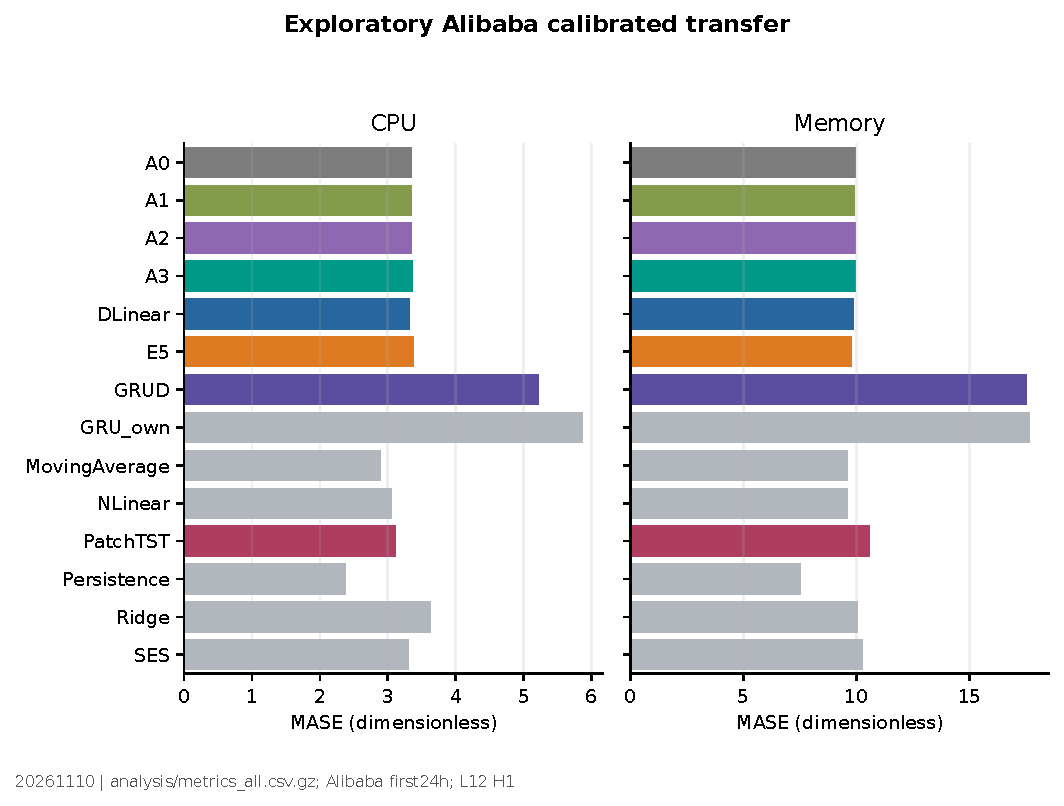
\includegraphics[width=0.79\textwidth]{figuras/12_external.pdf}
\caption{Exploratory first-day Alibaba transfer. Bars show MASE on 32 availability-selected services and 36 half-hour targets after a six-hour calibration prefix. These bars do not represent independent-infrastructure validation.}\label{fig:external}\end{figure*}

At L12, A3 uses 15 trainable parameters per resource versus DLinear's 26 and E5's 74. For a batch of one origin with 32 services, measured CPU p50 forward latency is 0.050 ms for A3, 0.057 ms for DLinear and 0.295 ms for E5; synchronized CUDA p50 is 0.141, 0.281 and 0.665 ms, respectively. PatchTST has 2499 trainable elements, CPU p50 0.521 ms and CUDA p50 1.212 ms. These samples show an observed accuracy/cost tradeoff under resident-input inference, not total monitoring latency or a causal hardware-wide speedup. On this small batch, CUDA is slower than CPU for some compact references. Completed-epoch time medians, including validation, are 8.56 s for A3, 10.21 s for DLinear, 14.72 s for E5 and 42.88 s for PatchTST; these exclude tuning, checkpoint I/O and failed incomplete attempts. Table~\ref{tab:efficiency} includes p95 values and all families. Fig.~\ref{fig:latency} relates the measured forward times to CPU error, and Fig.~\ref{fig:params} shows that a similar size can accompany different MASE values.
\begin{table*}[!t]
\caption{Trainable elements and measured p50/p95 forward latency in ms at B1/32 services. CUDA rows synchronize each trial; GRU-D CUDA uses replay without capture setup. Epoch sum is the median completed source-fit epoch-time sum over primary seeded fits, not total research time.}\label{tab:efficiency}
\centering\footnotesize
\FitTable{\begin{tabular}{lrrrrrr}
\toprule
Model & Parameters & CPU p50 & CPU p95 & CUDA p50 & CUDA p95 & Epoch sum (s) \\
\midrule
Persistence & 0 & 0.005 & 0.005 & 0.012 & 0.012 & not timed \\
Moving average & 0 & 0.014 & 0.015 & 0.023 & 0.025 & not timed \\
Exponential smoothing & 0 & 0.195 & 0.417 & 0.328 & 0.337 & not timed \\
Ridge & 13 & 0.022 & 0.024 & 0.084 & 0.092 & not timed \\
DLinear & 26 & 0.057 & 0.064 & 0.281 & 0.337 & 10.21 \\
NLinear & 13 & 0.031 & 0.045 & 0.095 & 0.102 & 7.62 \\
E5 & 74 & 0.295 & 0.317 & 0.665 & 0.681 & 14.72 \\
A0 & 13 & 0.022 & 0.023 & 0.085 & 0.095 & 7.26 \\
A1 & 14 & 0.046 & 0.049 & 0.125 & 0.134 & 7.99 \\
A2 & 14 & 0.030 & 0.032 & 0.104 & 0.116 & 7.10 \\
A3 & 15 & 0.050 & 0.056 & 0.141 & 0.166 & 8.56 \\
GRU (own) & 841 & 0.425 & 0.450 & 0.341 & 0.360 & 15.41 \\
GRU (graph) & 841 & 0.413 & 0.439 & 0.344 & 0.352 & 15.60 \\
GRU-D adaptation & 615 & 1.475 & 2.789 & 0.443 & 0.444 & 15.72 \\
PatchTST (small) & 2499 & 0.521 & 0.546 & 1.212 & 1.316 & 42.88 \\
\bottomrule
\end{tabular}
}
\end{table*}
\begin{figure*}[!t]\centering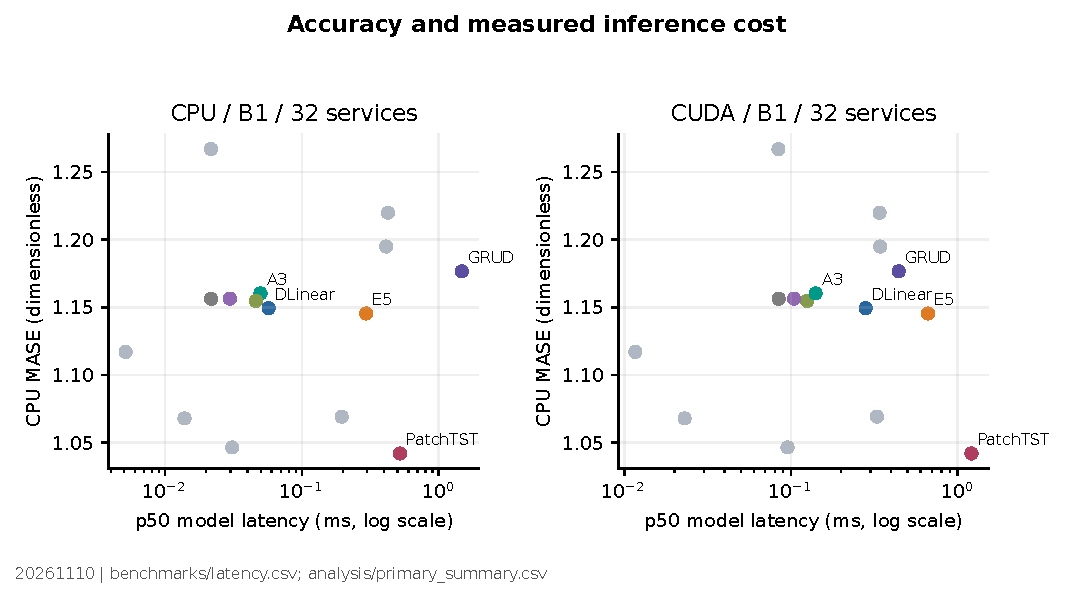
\includegraphics[width=0.79\textwidth]{figuras/13_latency.pdf}
\caption{CPU-resource MASE versus measured p50 forward latency. B1 inputs reside on the measured device. The laptop was shared, and these points exclude collection, preprocessing and control.}\label{fig:latency}\end{figure*}

\begin{figure*}[!t]\centering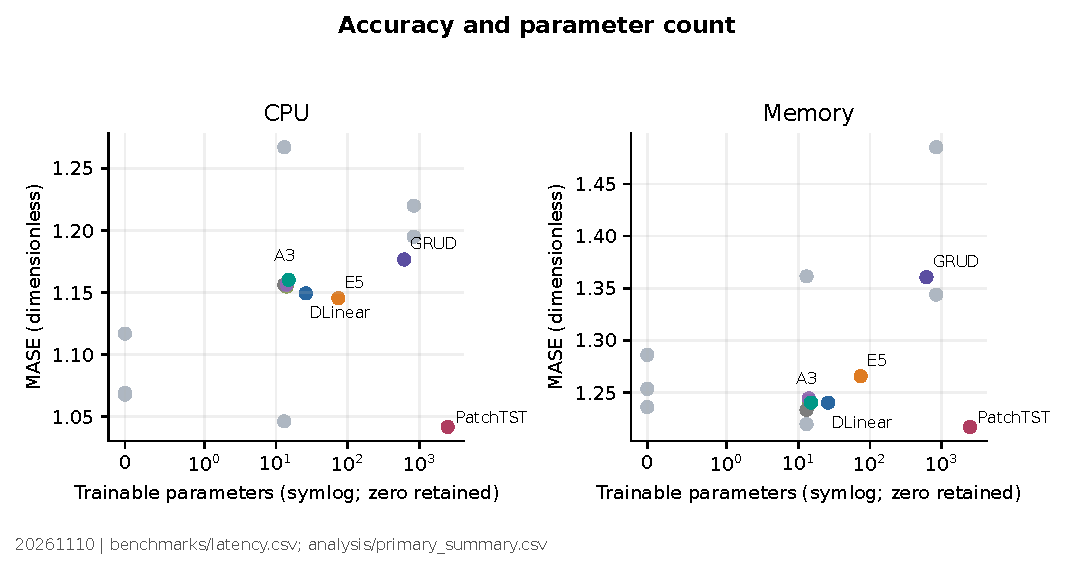
\includegraphics[width=0.79\textwidth]{figuras/14_parameters.pdf}
\caption{Error versus trainable count per resource. A symmetric-log axis retains zero-parameter references. Parameter counts exclude calibration and input state and therefore cannot substitute for measured memory or latency.}\label{fig:params}\end{figure*}

The resource monitor sampled one project-process RSS maximum of 1725.47 MiB; it did not capture a continuous peak. Whole-system RAM availability stayed above 10.87 GiB. Whole-system GPU memory in use reached 3536 MiB and the maximum recorded GPU temperature was $75^\circ$C; neither total can be attributed solely to our process. The CPU sensor reached $92^\circ$C and the study guard recorded one pause episode. The log retains seven failed GRU-D source attempts, 22 training OOM restart events and 94 inference batch-reduction events; the scheduled final fits and evaluations nonetheless have complete markers. Project energy was not measured.





\subsection{Integrated answers to the research questions}
Table~\ref{tab:rq} connects the five phases without averaging incompatible evidence. The historical memory gain motivates a model-design question; it is not added to the destination gain to obtain a larger effect. Similarly, the raw Alibaba download volume documents provenance and processing effort, while the inferential support is thirty-six targets per service. The numerical audit establishes consistency between saved predictions and reported errors, not independence from every unobserved preprocessing decision made by the data publisher.
\begin{table*}[!t]
\caption{Evidence-based answers. Directions are observed within the specified experiment, with the four primary sign tests reported separately.}\label{tab:rq}
\centering\footnotesize
\begin{tabularx}{\linewidth}{p{.08\linewidth}XXX}
\toprule RQ & Main evidence and direction & Scope & Limitation \\\midrule
1 & Original loss curves generally increase; prolonged blocks raise A3 error & Fixed traces and synthetic generators & Real outages and every service are not established \\
2 & Historical E5 improves memory, worsens CPU; fixed DLinear is affine & E/C/A parameterizations separately & Selection and optimization differ \\
3 & A3 does not beat A0 aggregate; E descriptors give mixed results & Independently tuned families & No orthogonal causal descriptor effect \\
4 & A3 uses15 vs26/74 parameters; lower measured forward cost & B1 resident tensors on measured CPU/CUDA & No universal accuracy/energy advantage \\
5 & PatchTST/NLinear lowest primary means; persistence best external MASE & Calibrated destination32 and one Alibaba day & No independent-period or population validation \\
6 & Historical crossed intervals widen; A3/E5 memory10/10 seeds & Fixed services, masks and selected configurations & Service concentration and temporal dependence remain \\
\bottomrule
\end{tabularx}
\end{table*}


\section{Discussion}\label{sec:discussion}
The compact A3 model demonstrates parameter reduction and an observed memory gain against E5 on these fixed new services. The broader evidence does not support a uniform accuracy improvement. CPU A3 is worse in mean MASE than both primary references, the A0 variant has lower memory MASE than A3, and the strongest mean MASE in the primary cohort belongs to the small PatchTST recipe. A3's favorable memory contrast is concentrated in a minority of services, although its seed direction is consistent under the prespecified fixed-cohort comparison. The outcome-informed service exclusions show why directional seed consistency alone does not imply broad spatial portability.

The algebraic result explains a practical boundary: a fixed MA decomposition followed by separate affine heads is itself affine. Reducing its parameterization can lower measured model-forward cost, but a different Adam trajectory and explicit availability coefficients can improve or worsen errors. E5's availability-dependent EMA is outside that exact collapse. The independently tuned A1/A2/A3 means do not demonstrate a general additive benefit from either simple missingness descriptor. A future mechanism study could hold hyperparameters fixed, evaluate descriptor interactions against matched regularization and use a longer independently sampled period; those are proposed experiments, not results here.

The external case changes both data domain and measurement definition. Its persistence advantage is consistent with a short, slowly changing normalized trace, but these observations do not establish the underlying cause. No external graph was available, and six calibration hours yield potentially small scale denominators. We therefore report external MASE and normalized absolute errors together, without combining their magnitudes with ChronoGraph physical errors. Additional days, independently chosen services and datasets with documented preprocessing would test whether any ranking persists.

The efficiency measurements add a useful but bounded perspective. A3 is much smaller than E5, and its resident-tensor p50 latency is lower on both measured devices. PatchTST offers lower primary mean MASE at a higher measured forward cost; simple moving average is a strong CPU accuracy reference with no trainable weights. In a small batch, CPU sometimes outperforms CUDA because launch and synchronization costs matter. None of these facts establishes lower energy, quicker telemetry collection or better operational autoscaling. A deployment trial would need a controller, workload replay, end-to-end timing, explicit SLA metrics and a reliable project-level power meter.

The preserved historical study should be read with its separate condition definitions. Its E5 memory ranking was a hypothesis source, not independent confirmation. The new spatial comparison demonstrates a material change in model ordering, and Alibaba changes it again. A severe historical GinAR error is retained as an implementation/protocol result and does not warrant a claim about the model's published behavior. The principal reproducible contribution is the transparent accounting of when compactness, error, missingness and domain transfer disagree.


The historical-to-expanded transition changes more than the number of seeds. The destination services have different per-service calibration, a different role in fitting, and a source training recipe that now includes ten conditions. E5's change in rank consequently cannot be attributed solely to having more services or initializations. Historical memory improvement, C-family failure to preserve it, and the new A3 contrast jointly answer the compactness question: reducing coefficients can retain an acceptable measured error while losing a specific earlier advantage, and a later favorable reference comparison does not restore universal superiority.

NLinear and PatchTST suggest that an explicit recent level or a learned patched representation can be competitive under source-trained transfer. The experiment does not isolate those mechanisms. Their selected optimization settings and parameterizations differ, and the PatchTST recipe contains normalization and attention together. Moreover, NLinear has slightly lower displayed CPU MAE than PatchTST despite the opposite MASE order. MASE weights errors relative to each service's training variability, whereas absolute macro errors weight the same physical unit. An algorithm ranking therefore depends on the scientific loss function as well as the cohort.

Longer direct horizons increase displayed errors for the selected learned models, but these endpoints use independently fitted weights and common target support. They are not evidence of recursive-error accumulation. Longer histories have mixed resource-specific effects: improved CPU A3 and worsened memory A3 are both retained. The counterexample matters because a longer window increases coefficients, input processing and possible exposure to older regimes. It cannot be assumed to improve generalization merely by containing more values. The star design describes these particular choices rather than estimating a complete interaction between every history and horizon.

Finally, the historical correction of interval units is scientifically substantive. An absolute MASE interval cannot be read as a percentage interval simply because it appears next to a percentage effect. In the expanded analysis, mean paired cell reductions and ratios of means remain explicitly separate. Likewise, the sign test measures seeded directional consistency and the conditional block interval describes a resampled mean. Agreement is informative, but disagreement is possible without an arithmetic error. These distinctions prevent narrow conditional uncertainty or a favorable rank from becoming an unsupported population-wide superiority claim.

The source training-only dynamics provide one check on the resource-specific interpretation. Median lag-one autocorrelation across the 28 series is 0.447 for CPU and 0.867 for memory. Median absolute change relative to series standard deviation is 0.413 and 0.275, respectively. This is compatible with more persistent memory levels. It cannot identify why the EMA changes forecast error, because the residual retains deviations from the estimated level and the two heads are fitted jointly. The observations motivate a controlled error analysis around abrupt changes rather than a claim that smoothing mechanically delays the final forecast.

\section{Threats to Validity}
\paragraph{Construct validity.} Recorded utilization is not unconstrained resource demand. ChronoGraph point samples and Alibaba completed-interval means have different semantics; external min--max values cannot be interpreted as bytes or cores. Synthetic losses affect inputs while complete recorded targets remain available. The masks simulate mechanisms rather than establish the incidence or cause of real monitoring outages. Calibration assumes the available historical prefix, not a fully missingness-degraded learning process. Availability descriptors and carry-forward summaries can retain information older than the nominal input window.

\paragraph{Internal validity.} Prefix-only normalization, partition/gap checks, future-perturbation tests for lag-MAR, fixed-mask hidden-value checks and saved-prediction audits address identifiable implementation risks. They do not certify all provider preprocessing. The external release's min--max scope and historical availability of static graph edges remain uncertain. Source validation chooses hyperparameters and stopping points; the destination prefix calibrates scale but does not fit weights. A narrow search budget, rotating neural condition exposure, full-condition analytic ridge fitting, different optimizer parameterizations and microbatch BatchNorm limit claims of equal optimization opportunity. The pretest GPU-memory amendment and recovered failures are retained, not concealed.

\paragraph{Statistical conclusion validity.} Services share a system, windows overlap and masks are paired. Seed replication estimates algorithm randomness on fixed data, not the number of independent infrastructures. The exact sign test concerns directional seed consistency, whereas the arithmetic mean difference is a separately reported effect. Source tuning reuses seed 101, addressed only by an explicitly exploratory leave-seed-out sensitivity. Conditional block-bootstrap intervals rely on a useful local block approximation; their sensitivity cannot establish universal temporal stationarity. Only four primary tests receive the prespecified multiplicity control; other patterns, horizons and cohorts are descriptive.

\paragraph{External validity.} The source and new ChronoGraph services share a period and infrastructure, the source test was historically inspected, and the destination cohort is topology-selected. Neither a local timestamped freeze nor exclusion from located earlier artifacts establishes third-party blinding. Alibaba contributes just one day, a six-hour calibration prefix and 36 target bins for 32 availability-selected services. Hundreds of millions of underlying pod records do not become hundreds of millions of independent forecast targets. Provider normalization and pod aggregation also change the task. Longer independent periods, other providers and workload regimes remain necessary before general cloud claims.

\paragraph{Efficiency and operational validity.} The laptop is shared; resident-tensor inference is not collector-to-controller latency. CPU and GPU timings depend on batch, synchronization, capture method and implementation. Parameter counts exclude state, calibration and orchestration costs. Sampled whole-system GPU memory includes other applications; process RSS is not a continuously observed peak. Epoch timing excludes some research and checkpoint costs and cannot identify a causal architecture-only training advantage. No controller, deployment, energy instrument or measured SLA benefit is available.


\section{Conclusions}
On the 32 additional ChronoGraph services, A3 reduced parameter count from 74 for E5 to 15 and improved memory MASE by 0.02523 under the prespecified fixed-cohort contrast (ten favorable seed means; Holm-adjusted $p=0.0078125$). It did not outperform DLinear in the primary mean, and its CPU mean was worse than both primary references. The small PatchTST configuration had the lowest observed primary mean MASE for CPU and memory, without a prespecified significance claim against NLinear. In the external first-day case, persistence had the lowest MASE for both resources. These results favor careful baseline selection and domain-sensitive interpretation over a universal missingness-architecture claim.

Further research requires independently timed cohorts and longer external periods, documented release preprocessing and graph availability, real interruption measurements, matched component interventions and measured controller outcomes. The local archive permits reconstruction of the numerical comparisons and their limits. Editorial use still requires both authors' final approval, a corresponding-author designation and decisions on prior-publication disclosure and authorized data/code release.
The historical phases supply a necessary part of this answer: E5's paired reduction was positive for memory (1.280\%) and negative for CPU ($-0.984\%$), and V2 did not retain the full memory benefit. The secondary extensions show increasing errors at longer direct horizons and mixed responses to larger histories. These findings make simple references and negative results central to model assessment rather than incidental exceptions.

\section*{Data and Code Availability}
Source code, configurations and summary metrics are available at \href{https://github.com/Nunclear/prediccion-proactiva-de-recursos-computacionales-para-microservicios}{public project repository}. Processed cohorts are distributed separately for academic review. Model weights, saved predictions and raw external objects remain in the local research archive. ChronoGraph and PatchTST retain their code licenses; Alibaba research-use terms do not establish unrestricted redistribution permission. Data use and redistribution must follow the owners\' terms.

\section*{Author Contributions}
Individual contributions have not yet been specified by the authors. CRediT roles and ORCID identifiers have not been inferred. Both named authors must review the final scientific text and approve the submission version before editorial use.
\section*{Funding}
This research received no external funding.
\section*{Conflicts of Interest}
The authors declare no conflicts of interest.
\section*{Prior-version status}
The local materials establish that a historical manuscript exists, but do not establish whether it remained internal, was an academic submission, a preprint, under review, accepted or published. This status must be confirmed by the authors before submission; any existing public version or publication requires the appropriate citation and disclosure of overlap. No editorial status has been inferred from a local PDF.

\FloatBarrier
\appendices
\section{Supplementary detailed comparisons}
\subsection{All added stress conditions and variability}
Table~\ref{tab:stress} retains all model families in correlated, prolonged and lag-MAR conditions. Table~\ref{tab:variation} separates variation across seed means and mask means. A seed standard deviation is undefined for a deterministic reference with one fit; it is not silently set to zero.
\begin{table*}[!t]
\caption{Descriptive MASE under the three additional missingness mechanisms. ``Long'' denotes prolonged blocks; lag-MAR uses a nominal label with variable realized rate.}\label{tab:stress}
\centering\footnotesize
\FitTable{\begin{tabular}{lrrrrrr}
\toprule
Model & CPU corr. & CPU long & CPU lag-MAR & Mem. corr. & Mem. long & Mem. lag-MAR \\
\midrule
Persistence & 1.0836 & 1.2113 & 1.0934 & 1.2422 & 1.4198 & 1.2493 \\
Moving average & 1.0326 & 1.1509 & 1.0521 & 1.1885 & 1.3576 & 1.2091 \\
Exponential smoothing & 1.0332 & 1.1470 & 1.0522 & 1.2024 & 1.3700 & 1.2254 \\
Ridge & 1.2453 & 1.3294 & 1.2518 & 1.3217 & 1.4826 & 1.3355 \\
DLinear & 1.1235 & 1.2222 & 1.1326 & 1.1956 & 1.3701 & 1.2120 \\
NLinear & 1.0121 & 1.1375 & 1.0281 & 1.1737 & 1.3532 & 1.1902 \\
E5 & 1.1194 & 1.2187 & 1.1300 & 1.2250 & 1.4072 & 1.2452 \\
A0 & 1.1300 & 1.2285 & 1.1393 & 1.1881 & 1.3638 & 1.2048 \\
A1 & 1.1285 & 1.2273 & 1.1377 & 1.1942 & 1.3701 & 1.2109 \\
A2 & 1.1299 & 1.2289 & 1.1393 & 1.1985 & 1.3783 & 1.2151 \\
A3 & 1.1342 & 1.2330 & 1.1428 & 1.1932 & 1.3743 & 1.2106 \\
GRU (own) & 1.1879 & 1.3095 & 1.2019 & 1.2932 & 1.5458 & 1.3110 \\
GRU (graph) & 1.1603 & 1.2816 & 1.1761 & 1.4235 & 1.7076 & 1.4393 \\
GRU-D adaptation & 1.1394 & 1.2605 & 1.1592 & 1.3076 & 1.5114 & 1.3286 \\
PatchTST (small) & 1.0053 & 1.1323 & 1.0223 & 1.1712 & 1.3485 & 1.1894 \\
\bottomrule
\end{tabular}
}
\end{table*}
\begin{table*}[!t]
\caption{Primary positive-loss MASE standard deviations across seed means and mask means. These two conditional summaries are not independent population variance components.}\label{tab:variation}
\centering\footnotesize
\FitTable{\begin{tabular}{lrrrr}
\toprule
Model & CPU seed SD & CPU mask SD & Memory seed SD & Memory mask SD \\
\midrule
Persistence & undefined & 0.0033 & undefined & 0.0065 \\
Moving average & undefined & 0.0031 & undefined & 0.0062 \\
Exponential smoothing & undefined & 0.0034 & undefined & 0.0082 \\
Ridge & undefined & 0.0021 & undefined & 0.0063 \\
DLinear & 0.0332 & 0.0023 & 0.0161 & 0.0062 \\
NLinear & 0.0081 & 0.0030 & 0.0112 & 0.0062 \\
E5 & 0.0227 & 0.0025 & 0.0179 & 0.0066 \\
A0 & 0.0265 & 0.0024 & 0.0126 & 0.0063 \\
A1 & 0.0238 & 0.0024 & 0.0215 & 0.0063 \\
A2 & 0.0262 & 0.0024 & 0.0179 & 0.0063 \\
A3 & 0.0222 & 0.0024 & 0.0154 & 0.0063 \\
GRU (own) & 0.0634 & 0.0018 & 0.0341 & 0.0050 \\
GRU (graph) & 0.0313 & 0.0022 & 0.0403 & 0.0051 \\
GRU-D adaptation & 0.0426 & 0.0020 & 0.0463 & 0.0050 \\
PatchTST (small) & 0.0093 & 0.0030 & 0.0105 & 0.0062 \\
\bottomrule
\end{tabular}
}
\end{table*}

\subsection{Conditional block sensitivity and common-support extensions}
\begin{table}[!t]
\caption{95\% crossed seed/mask/circular-block bootstrap intervals for $\Delta$MASE, reference minus A3. Block lengths 24/48/96 correspond to 12/24/48 nominal hours. No infrastructure-population or predictive coverage is asserted.}\label{tab:block}
\centering\footnotesize
\FitTable{\begin{tabular}{lrrrr}
\toprule
Resource & Reference & Block steps & Lower & Upper \\
\midrule
CPU & DLinear & 24 & -0.02818 & 0.00581 \\
CPU & DLinear & 48 & -0.02732 & 0.00470 \\
CPU & DLinear & 96 & -0.02944 & 0.00518 \\
CPU & E5 & 24 & -0.02903 & -0.00094 \\
CPU & E5 & 48 & -0.02977 & -0.00120 \\
CPU & E5 & 96 & -0.02966 & -0.00011 \\
Memory & DLinear & 24 & -0.01024 & 0.01019 \\
Memory & DLinear & 48 & -0.00959 & 0.01035 \\
Memory & DLinear & 96 & -0.00988 & 0.00981 \\
Memory & E5 & 24 & 0.01264 & 0.03961 \\
Memory & E5 & 48 & 0.01312 & 0.03981 \\
Memory & E5 & 96 & 0.01233 & 0.03971 \\
\bottomrule
\end{tabular}
}
\end{table}
\begin{table*}[!t]
\caption{Common-target-origin MASE for CPU (left) and memory (right), with horizons in minutes. Three seeds and five masks, six original positive-loss conditions; H30 here is a subset of the primary endpoint.}\label{tab:horizon}
\centering\footnotesize

\setlength{\tabcolsep}{4pt}
\begin{minipage}[t]{.485\textwidth}
\centering\FitTable{\begin{tabular}{lrrrrr}
\toprule
Model & 30 & 60 & 120 & 180 & 360 \\
\midrule
Persistence & 1.1159 & 1.1381 & 1.3408 & 1.4851 & 1.7819 \\
Moving average & 1.0666 & 1.1420 & 1.3589 & 1.4831 & 1.7010 \\
Exponential smoothing & 1.0686 & 1.1469 & 1.3009 & 1.4242 & 1.6651 \\
Ridge & 1.2672 & 1.3856 & 1.6037 & 1.7441 & 2.0420 \\
DLinear & 1.1453 & 1.2419 & 1.4287 & 1.6340 & 1.9346 \\
E5 & 1.1384 & 1.2541 & 1.4506 & 1.6121 & 1.9251 \\
A3 & 1.1584 & 1.2492 & 1.4448 & 1.6451 & 1.9779 \\
PatchTST (small) & 1.0445 & 1.1217 & 1.2814 & 1.4077 & 1.6399 \\
\bottomrule
\end{tabular}
}
\end{minipage}
\hfill
\begin{minipage}[t]{.485\textwidth}
\centering\FitTable{\begin{tabular}{lrrrrr}
\toprule
Model & 30 & 60 & 120 & 180 & 360 \\
\midrule
Persistence & 1.2862 & 1.3398 & 1.6072 & 1.8097 & 2.2313 \\
Moving average & 1.2364 & 1.3384 & 1.6286 & 1.7971 & 2.2460 \\
Exponential smoothing & 1.2544 & 1.3549 & 1.5611 & 1.7315 & 2.1303 \\
Ridge & 1.3640 & 1.5179 & 1.8084 & 2.0411 & 2.5289 \\
DLinear & 1.2528 & 1.3958 & 1.6037 & 1.8014 & 2.3050 \\
E5 & 1.2680 & 1.4250 & 1.6459 & 1.8648 & 2.3222 \\
A3 & 1.2436 & 1.3474 & 1.6060 & 1.8353 & 2.3141 \\
PatchTST (small) & 1.2264 & 1.3377 & 1.5866 & 1.7572 & 2.1681 \\
\bottomrule
\end{tabular}
}
\end{minipage}
\end{table*}
\begin{table*}[!t]
\caption{Common-target-origin MASE for CPU (left) and memory (right), with history in half-hour steps at horizon 30 minutes. This secondary star design is descriptive.}\label{tab:history}
\centering\footnotesize

\setlength{\tabcolsep}{4pt}
\begin{minipage}[t]{.485\textwidth}
\centering\FitTable{\begin{tabular}{lrrr}
\toprule
Model & 12 & 24 & 48 \\
\midrule
Persistence & 1.1159 & 1.1159 & 1.1159 \\
Moving average & 1.0666 & 1.0666 & 1.0666 \\
Exponential smoothing & 1.0686 & 1.0625 & 1.0618 \\
Ridge & 1.2672 & 1.2403 & 1.1504 \\
DLinear & 1.1453 & 1.1372 & 1.1072 \\
E5 & 1.1384 & 1.1402 & 1.1071 \\
A3 & 1.1584 & 1.1572 & 1.0966 \\
PatchTST (small) & 1.0445 & 1.0421 & 1.0618 \\
\bottomrule
\end{tabular}
}
\end{minipage}
\hfill
\begin{minipage}[t]{.485\textwidth}
\centering\FitTable{\begin{tabular}{lrrr}
\toprule
Model & 12 & 24 & 48 \\
\midrule
Persistence & 1.2862 & 1.2862 & 1.2862 \\
Moving average & 1.2364 & 1.2364 & 1.2364 \\
Exponential smoothing & 1.2544 & 1.2501 & 1.2494 \\
Ridge & 1.3640 & 1.3385 & 1.3063 \\
DLinear & 1.2528 & 1.2543 & 1.2610 \\
E5 & 1.2680 & 1.2680 & 1.2681 \\
A3 & 1.2436 & 1.2521 & 1.2560 \\
PatchTST (small) & 1.2264 & 1.2190 & 1.2413 \\
\bottomrule
\end{tabular}
}
\end{minipage}
\end{table*}

\subsection{Complete external and historical summaries}
\begin{table*}[!t]
\caption{Exploratory Alibaba transfer: six original positive-loss conditions. Absolute MAE/RMSE use the provider's normalized utilization for both resources. They must not be read as CPU cores or memory bytes.}\label{tab:external}
\centering\footnotesize
\FitTable{\begin{tabular}{lrrrrrr}
\toprule
Model & CPU MASE & CPU MAE & CPU RMSE & Mem. MASE & Mem. MAE & Mem. RMSE \\
\midrule
Persistence & 2.3795 & 0.007548 & 0.011324 & 7.5150 & 0.001085 & 0.002302 \\
Moving average & 2.8906 & 0.009822 & 0.013787 & 9.6034 & 0.001392 & 0.002726 \\
Exponential smoothing & 3.3095 & 0.011482 & 0.015495 & 10.2802 & 0.001847 & 0.003271 \\
Ridge & 3.6334 & 0.012690 & 0.016598 & 10.0263 & 0.001885 & 0.003208 \\
DLinear & 3.3262 & 0.011559 & 0.015422 & 9.8853 & 0.001762 & 0.003090 \\
NLinear & 3.0566 & 0.010455 & 0.014191 & 9.5989 & 0.001658 & 0.002972 \\
E5 & 3.3842 & 0.011791 & 0.015759 & 9.7985 & 0.001767 & 0.003104 \\
A0 & 3.3521 & 0.011664 & 0.015584 & 9.9413 & 0.001760 & 0.003097 \\
A1 & 3.3481 & 0.011650 & 0.015572 & 9.9291 & 0.001759 & 0.003095 \\
A2 & 3.3520 & 0.011663 & 0.015584 & 9.9668 & 0.001780 & 0.003117 \\
A3 & 3.3593 & 0.011686 & 0.015601 & 9.9535 & 0.001768 & 0.003105 \\
GRU (own) & 5.8743 & 0.020136 & 0.024363 & 17.6403 & 0.004010 & 0.006199 \\
GRU-D adaptation & 5.2232 & 0.017836 & 0.022202 & 17.5279 & 0.003966 & 0.006144 \\
PatchTST (small) & 3.1112 & 0.010653 & 0.015257 & 10.5876 & 0.001559 & 0.002796 \\
\bottomrule
\end{tabular}
}
\end{table*}
The seven-condition historical means in Table~\ref{tab:historical} retain complete telemetry. Table~\ref{tab:matrix} documents the scope of the expanded run without treating repeated metric rows as independent observations.
\begin{table}[!t]
\caption{Preserved historical cohort: MASE averaged over all seven original conditions, including complete telemetry. These means have a different condition scope from the new primary positive-loss endpoint. V2 is a validation-selected alias of existing compact fits. Extreme GinAR values remain visible and characterize this implementation/protocol, not a canonical-model refutation.}\label{tab:historical}
\centering\footnotesize
\FitTable{\begin{tabular}{lrr}
\toprule
Historical model & CPU MASE & Memory MASE \\
\midrule
persistencia & 1.0761 & 1.3112 \\
E0 & 0.9874 & 1.1283 \\
GRU\_propia & 0.9495 & 1.1580 \\
GRU\_llamadas & 0.9324 & 1.1893 \\
GinAR & 704115.0298 & 2.5812 \\
BiTGraph\_codigo\_autor & 0.9914 & 1.2009 \\
E1 & 1.0179 & 1.1283 \\
E2 & 1.0170 & 1.1178 \\
E3 & 0.9994 & 1.1267 \\
E4 & 0.9852 & 1.1283 \\
E5 & 0.9979 & 1.1136 \\
C0 & 1.0170 & 1.1283 \\
C1 & 1.0168 & 1.1278 \\
C2 & 1.0171 & 1.1284 \\
C3 & 1.0168 & 1.1280 \\
V2 & 1.0168 & 1.1278 \\
\bottomrule
\end{tabular}
}
\end{table}
\begin{table}[!t]
\caption{Executed metric matrix. Rows count repeated service summaries across models, seeds, masks and conditions. They are not independent datasets.}\label{tab:matrix}
\centering\footnotesize
\FitTable{\begin{tabular}{lrrrrr}
\toprule
Dataset & L & h steps & Models & Masks & Metric rows \\
\midrule
alibaba\_transfer & 12 & 1 & 14 & 20 & 1331200 \\
new\_services & 12 & 1 & 15 & 20 & 1459200 \\
new\_services & 12 & 2 & 8 & 5 & 51200 \\
new\_services & 12 & 4 & 8 & 5 & 51200 \\
new\_services & 12 & 6 & 8 & 5 & 51200 \\
new\_services & 12 & 12 & 8 & 5 & 51200 \\
new\_services & 24 & 1 & 8 & 5 & 51200 \\
new\_services & 48 & 1 & 8 & 5 & 51200 \\
\bottomrule
\end{tabular}
}
\end{table}

\section{Reconstruction and Provenance}
The local \path{results/analysis/prediction_manifest.csv} records every new prediction file and its array/file digests; \path{checkpoint_manifest.csv} records checkpoint hashes and predictor fingerprints. \path{metrics_all.csv.gz} retains full numerical precision and explicit target semantics. Table display rounding never changes those source records. \path{tablas/provenance.json} and the figure manifest specify filters and sources. The source-code hash list in the local frozen protocol is checked again during analysis.

The analyzer independently reconstructs float64 physical-unit metric equations, target counts and chronological indices from saved prediction arrays. Mask regeneration uses the frozen generator and is therefore a consistency check rather than a second independent mask algorithm. Unit tests cover boundary/gap exclusion, future-prefix invariance for lag-MAR, one fixed-mask hidden-value perturbation, provenance identities, finite CPU/CUDA model behavior and affine initialization. Same-backend interruption/replay tests address checkpoint recovery and the CUDA optimization. These checks are targeted evidence; they do not prove universal absence of data leakage in provider releases.

The derived Docker image reuses a preserved local research base. Its image identifiers and dependency freeze are recorded, but a fresh independent-machine build is not certified. Process CPU sampling was corrected after an initialization defect: earlier RSS values remain valid, earlier CPU zeros are excluded, and the amendment is preserved. Epoch timing, sampled RSS, Torch allocation and whole-system telemetry keep separate definitions. The accompanying README documents the actual execution and commands for bounded reconstruction without retuning.

\subsection{Separate memory and historical timing measurements}
Table~\ref{tab:historical-bench} preserves selected CUDA B128 measurements on source28. Table~\ref{tab:memory-bench} reports B1 CUDA inference measurements on destination32 for the CPU forecasting target. RSS describes process memory, whereas peak CUDA allocation describes the PyTorch allocator. Baselines and context differ across protocols, and neither metric should be used as a parameter-size conversion.
\begin{table}[!t]
\caption{Historical B128 CUDA eager, seed101. RSS is the reported process peak and CUDA is peak allocated memory. Seconds include training and validation for the corresponding fit.}\label{tab:historical-bench}
\centering\footnotesize
\FitTable{\begin{tabular}{lrrrrr}
\toprule
Model / resource & p50 (ms) & p95 (ms) & RSS (MiB) & CUDA (MiB) & s \\
\midrule
E0 / Memory & 0.287 & 0.602 & 840.2 & 64.84 & 7.805 \\
E2 / Memory & 0.595 & 0.692 & 849.6 & 64.21 & 5.199 \\
E4 / Memory & 0.441 & 0.937 & 889.8 & 64.51 & 5.295 \\
E5 / Memory & 0.801 & 0.869 & 930.7 & 77.35 & 6.342 \\
V2 / Memory & 0.416 & 0.556 & 914.1 & 64.51 & 4.630 \\
E0 / CPU & 0.284 & 0.483 & 839.7 & 64.84 & 12.799 \\
E2 / CPU & 0.585 & 0.681 & 848.7 & 64.21 & 9.521 \\
E4 / CPU & 0.432 & 0.675 & 889.2 & 64.51 & 15.421 \\
E5 / CPU & 0.814 & 0.936 & 930.8 & 77.35 & 7.473 \\
V2 / CPU & 0.691 & 0.767 & 860.4 & 64.21 & 5.999 \\
\bottomrule
\end{tabular}
}
\end{table}
\begin{table}[!t]
\caption{Expanded CUDA B1/32 services. RSS is observed process memory and CUDA is allocator peak, both in MiB. GRU-D uses verified replay. Shared device totals are reported separately.}\label{tab:memory-bench}
\centering\footnotesize
\FitTable{\begin{tabular}{lrr}
\toprule
Model & RSS (MiB) & CUDA (MiB) \\
\midrule
A0 & 1160.49 & 114.861 \\
A1 & 1157.96 & 114.862 \\
A2 & 1160.36 & 114.861 \\
A3 & 1160.38 & 114.862 \\
DLinear & 1160.27 & 114.866 \\
E5 & 1157.80 & 114.877 \\
GRU-D adaptation & 1136.98 & 114.875 \\
GRU (graph) & 1160.43 & 123.216 \\
GRU (own) & 1157.50 & 123.216 \\
Moving average & 1137.01 & 114.865 \\
NLinear & 1157.62 & 114.861 \\
PatchTST (small) & 1096.40 & 82.992 \\
Persistence & 1137.00 & 114.859 \\
Ridge & 1157.65 & 114.861 \\
Exponential smoothing & 1160.39 & 114.860 \\
\bottomrule
\end{tabular}
}
\end{table}

\FloatBarrier
\bibliographystyle{IEEEtran}
\bibliography{referencias}
\end{document}
